\documentclass[12pt]{report}

% ============================================================
% BODY FORMATTING -- per the official Phase-1 Report Guidelines:
%  - A4 paper, margins L 1.25in, R 1in, T/B 0.75in
%  - 1.5 line spacing throughout
%  - Chapter number ("CHAPTER N"): 16pt, RIGHT justified
%  - Chapter title: 18pt, centered
%  - Section number+heading: 14pt, left justified, UPPERCASE
%  - Sub-section number+heading: 12pt, left justified
%  - Body text: 12pt, fully justified
%  - 10pt spacing between paragraphs
%  - No paragraph indentation
% ============================================================

\usepackage[a4paper,
  includehead,
  includefoot,
  left=1.25in,
  right=1in,
  top=0.75in,
  bottom=0.75in,
  headheight=22pt,
  headsep=12pt,
  footskip=30pt
]{geometry}

\usepackage[utf8]{inputenc}
\usepackage[T1]{fontenc}
\usepackage{setspace}
\usepackage{titlesec}
\usepackage{enumitem}
\usepackage{xcolor}
\usepackage{fancyhdr}
\usepackage{iftex}
\usepackage{graphicx}
\usepackage{longtable}
\usepackage{listings}
\usepackage{tikz}
\usepackage{float}
\usepackage{amsmath, amssymb, amsfonts}
\usepackage{booktabs}
\usepackage{tabularx}
\usepackage{array}
\usepackage{cite}
\usepackage[hidelinks, colorlinks=true, linkcolor=vcetmaroon, citecolor=vcetmaroon, urlcolor=vcetmaroon]{hyperref}
\usetikzlibrary{positioning,arrows.meta}

% ============================================================
% TIMES NEW ROMAN FONT SETUP
% ============================================================

\ifPDFTeX
  % pdfLaTeX
  \usepackage{times}
\else
  % XeLaTeX / LuaLaTeX
  \usepackage{fontspec}
  \setmainfont{Times New Roman}
\fi

% ============================================================
% PARAGRAPH FORMATTING
% ============================================================

\onehalfspacing

% No paragraph indentation
\setlength{\parindent}{0pt}

% 10pt spacing between paragraphs
\setlength{\parskip}{10pt}

% ============================================================
% PREVENT WORDS FROM BEING SPLIT WITH HYPHENS
% ============================================================

\usepackage[none]{hyphenat}

% Improve justification and character spacing
\usepackage{microtype}

% Tell LaTeX to adjust spacing rather than break words
\hyphenpenalty=10000
\exhyphenpenalty=10000

% Give LaTeX additional flexibility for justified paragraphs
\emergencystretch=3em

% ============================================================
% MAROON COLOUR
% ============================================================

\definecolor{vcetmaroon}{RGB}{99,36,35}

% ============================================================
% GRAPHICS PATH & SAFE IMAGE FALLBACK
% If an image is missing, render a neat box instead of aborting compile
% ============================================================

\graphicspath{{figures/}{./}}

\makeatletter
\let\oldincludegraphics\includegraphics
\renewcommand{\includegraphics}[2][]{%
  \IfFileExists{#2}{%
    \oldincludegraphics[#1]{#2}%
  }{%
    \IfFileExists{figures/#2}{%
      \oldincludegraphics[#1]{figures/#2}%
    }{%
      \fbox{\parbox[c][2.2cm][c]{0.7\linewidth}{\centering\small\bfseries\color{vcetmaroon}[Image File Missing: #2]}}%
    }%
  }%
}
\makeatother

% ============================================================
% LISTINGS CONFIGURATION
% ============================================================

\lstset{
  basicstyle=\ttfamily\small,
  breaklines=true,
  frame=single,
  numbers=left,
  numberstyle=\tiny\color{gray},
  keywordstyle=\bfseries\color{vcetmaroon},
  commentstyle=\color{gray!80!black},
  stringstyle=\color{teal},
  showstringspaces=false
}

% ============================================================
% HEADER / FOOTER CONTENT
% ============================================================

\newcommand{\reporttitle}
{Smart Mobile-Based Driving Behaviour \& Risk Monitoring System}

\newcommand{\reportyear}
{2026-27}

\newcommand{\deptline}
{Department of CSE (Data Science), VCET, Puttur}

% ============================================================
% HEADER / FOOTER
% ============================================================

\pagestyle{fancy}

\fancyhf{}

\renewcommand{\headrulewidth}{0pt}
\renewcommand{\footrulewidth}{0pt}

\fancyhead[L]{%
  \hspace*{0pt}%
  \normalfont\fontsize{11}{13}\selectfont
  \reporttitle
}

\fancyhead[R]{%
  \hspace*{5pt}%
  \normalfont\fontsize{11}{13}\selectfont
  \reportyear
}

\fancyfoot[L]{%
  \hspace*{0pt}%
  \normalfont\fontsize{11}{13}\selectfont
  \deptline
}

\fancyfoot[R]{%
  \hspace*{5pt}%
  \normalfont\fontsize{11}{13}\selectfont
  Page \thepage
}

% ============================================================
% DOUBLE RULE BELOW HEADER
% ============================================================

\renewcommand{\headrule}{%
  {\color{vcetmaroon}
   \hrule height 0.6pt width \headwidth}%
  \vskip 1pt
  {\color{vcetmaroon}
   \hrule height 3pt width \headwidth}%
}

% ============================================================
% DOUBLE RULE ABOVE FOOTER
% ============================================================

\renewcommand{\footrule}{%
  {\color{vcetmaroon}
   \hrule height 3pt width \headwidth}%
  \vskip 1pt
  {\color{vcetmaroon}
   \hrule height 0.6pt width \headwidth}%
}

% ============================================================
% PLAIN PAGE STYLE
% ============================================================

\fancypagestyle{plain}{%
  \fancyhf{}

  \fancyhead[L]{
    \normalfont
    \fontsize{11}{13}
    \selectfont
    \reporttitle
  }

  \fancyhead[R]{
    \normalfont
    \fontsize{11}{13}
    \selectfont
    \reportyear
  }

  \fancyfoot[L]{
    \normalfont
    \fontsize{11}{13}
    \selectfont
    \deptline
  }

  \fancyfoot[R]{
    \normalfont
    \fontsize{11}{13}
    \selectfont
    Page \thepage
  }

  \renewcommand{\headrulewidth}{0pt}
  \renewcommand{\footrulewidth}{0pt}

  \renewcommand{\headrule}{%
    {\color{vcetmaroon}
     \hrule height 0.6pt width \headwidth}%
    \vskip 1pt
    {\color{vcetmaroon}
     \hrule height 3pt width \headwidth}%
  }

  \renewcommand{\footrule}{%
    {\color{vcetmaroon}
     \hrule height 3pt width \headwidth}%
    \vskip 1pt
    {\color{vcetmaroon}
     \hrule height 0.6pt width \headwidth}%
  }
}

% ============================================================
% CHAPTER FORMAT
% ============================================================

\titleformat{\chapter}[display]
  {\bfseries\fontsize{16}{0}\selectfont\raggedleft}
  {CHAPTER \thechapter}
  {0pt}
  {\centering\bfseries\fontsize{18}{20}\selectfont}

\titlespacing*{\chapter}
  {0pt}
  {-10pt}
  {10pt}

% ============================================================
% SECTION FORMAT
% ============================================================

\titleformat{\section}
  {\normalfont\bfseries\fontsize{14}{19}\selectfont}
  {\thesection}
  {10pt}
  {\MakeUppercase}

\titlespacing*{\section}
  {0pt}
  {0pt}
  {5pt}

% ============================================================
% SUBSECTION FORMAT
% ============================================================

\titleformat{\subsection}
  {\normalfont\bfseries\fontsize{12}{17}\selectfont}
  {\thesubsection}
  {10pt}
  {}

\titlespacing*{\subsection}
  {0pt}
  {10pt}
  {-5pt}

\makeatletter
\renewcommand\@secpenalty{-50}
\makeatother

% ============================================================
% DOCUMENT
% ============================================================

\begin{document}

% ------------------------------------------------------------------------------
% PAGE 1: TITLE PAGE
% ------------------------------------------------------------------------------
\begin{titlepage}
    \centering
    {\large \textbf{\textcolor{vcetmaroon}{VISVESVARAYA TECHNOLOGICAL UNIVERSITY}}}\\[0.15cm]
    {\normalsize \textbf{JNANA SANGAMA, BELAGAVI -- 590 018, KARNATAKA, INDIA}}\\[0.6cm]
    
    
\includegraphics[width=2.5cm]{figures/vtu_logo.png}\\[0.5cm]
    
    {\large \textbf{A PROJECT REPORT (PHASE-1)}}\\[0.1cm]
    {\normalsize \textbf{ON}}\\[0.25cm]
    {\Large \textbf{\textcolor{vcetmaroon}{``SMART MOBILE-BASED DRIVING BEHAVIOUR \& RISK MONITORING SYSTEM''}}}\\[0.5cm]
    
    {\normalsize Submitted in partial fulfillment of the requirements for the award of}\\[0.12cm]
    {\large \textbf{BACHELOR OF ENGINEERING}}\\[0.08cm]
    {\normalsize in}\\[0.08cm]
    {\large \textbf{CSE (DATA SCIENCE)}}\\[0.5cm]
    
    {\normalsize \textbf{Submitted By}}\\[0.2cm]
    \begin{tabular}{cc}
        \textbf{Name} & \textbf{USN} \\
        PRANAV K U & [4VP23CD0XX] \\
        \lbrack Candidate Name 2\rbrack & \lbrack USN 2\rbrack \\
        \lbrack Candidate Name 3\rbrack & \lbrack USN 3\rbrack \\
        \lbrack Candidate Name 4\rbrack & \lbrack USN 4\rbrack \\
    \end{tabular}\\[0.5cm]
    
    {\normalsize \textbf{Under the Guidance of}}\\[0.1cm]
    {\large \textbf{\lbrack Guide Name\rbrack}}\\[0.05cm]
    {\normalsize \lbrack Designation\rbrack, Department of CSE (Data Science)}\\[0.5cm]
    
    
\includegraphics[width=2.2cm]{figures/vcet_logo.png}\\[0.35cm]
    
    {\large \textbf{\textcolor{vcetmaroon}{DEPARTMENT OF CSE (DATA SCIENCE)}}}\\[0.1cm]
    {\normalsize \textbf{VIVEKANANDA COLLEGE OF ENGINEERING \& TECHNOLOGY}}\\[0.05cm]
    {\footnotesize [A Unit of Vivekananda Vidyavardhaka Sangha, Puttur (R)]}\\[0.05cm]
    {\footnotesize Affiliated to Visvesvaraya Technological University and Approved by AICTE New Delhi \& Govt. of Karnataka}\\[0.05cm]
    {\footnotesize Nehru Nagara, Puttur -- 574 203, DK, Karnataka, India}\\[0.1cm]
    {\normalsize \textbf{Academic Year 2026 -- 2027}}
\end{titlepage}

% ------------------------------------------------------------------------------
% PAGE 2: CERTIFICATE
% ------------------------------------------------------------------------------
\newpage
\thispagestyle{empty}
\begin{center}
    {\large \textbf{\textcolor{vcetmaroon}{VIVEKANANDA COLLEGE OF ENGINEERING \& TECHNOLOGY}}}\\[0.05cm]
    {\footnotesize [A Unit of Vivekananda Vidyavardhaka Sangha, Puttur (R)]}\\[0.05cm]
    {\footnotesize Affiliated to Visvesvaraya Technological University and Approved by AICTE New Delhi \& Govt. of Karnataka}\\[0.05cm]
    {\footnotesize Nehru Nagara, Puttur -- 574 203, DK, Karnataka, India}\\[0.25cm]
    
    {\normalsize \textbf{\textcolor{vcetmaroon}{DEPARTMENT OF CSE (DATA SCIENCE)}}}\\[0.25cm]
    
    
\includegraphics[width=2.1cm]{figures/vcet_logo.png}\\[0.25cm]
    
    {\Large \textbf{CERTIFICATE}}\\[0.35cm]
\end{center}

\noindent Certified that the project work entitled \textbf{``Smart Mobile-Based Driving Behaviour \& Risk Monitoring System''} is carried out by \textbf{PRANAV K U, \lbrack Candidate Name 2\rbrack, \lbrack Candidate Name 3\rbrack, and \lbrack Candidate Name 4\rbrack} bearing USNs \textbf{\lbrack USN 1\rbrack, \lbrack USN 2\rbrack, \lbrack USN 3\rbrack\ and \lbrack USN 4\rbrack}, respectively bonafide students of \textbf{Vivekananda College of Engineering \& Technology}, in partial fulfillment for the award of \textbf{Bachelor of Engineering in CSE (Data Science)} of the \textbf{Visvesvaraya Technological University, Belagavi} during the year 2026-27. It is certified that all corrections / suggestions indicated for Internal Assessment have been incorporated in the report deposited in the departmental library.

\vspace{0.3cm}
\noindent The project report has been approved as it satisfies the academic requirements in respect of Project work prescribed for the said Degree.

\vspace{1.2cm}
\noindent
\begin{minipage}{0.32\textwidth}
    \centering
    \textbf{Signature of Guide}\\
    \textbf{\lbrack Guide Name\rbrack}\\
    \lbrack Designation\rbrack
\end{minipage}
\hfill
\begin{minipage}{0.32\textwidth}
    \centering
    \textbf{Signature of HOD}\\
    \textbf{\lbrack HOD Name\rbrack}\\
    Head of Department
\end{minipage}
\hfill
\begin{minipage}{0.32\textwidth}
    \centering
    \textbf{Signature of Principal}\\
    \textbf{\lbrack Principal Name\rbrack}\\
    Principal
\end{minipage}

\vspace{1.2cm}
\begin{center}
    \textbf{\large EXTERNAL VIVA}
\end{center}
\vspace{0.2cm}
\noindent
\begin{tabularx}{\textwidth}{lX}
    \textbf{Name of the Examiners} & \textbf{Signature with date} \\[0.5cm]
    1. ............................................................ & .................................................... \\[0.5cm]
    2. ............................................................ & .................................................... \\
\end{tabularx}

% ------------------------------------------------------------------------------
% PAGE 3: DECLARATION
% ------------------------------------------------------------------------------
\newpage
\thispagestyle{empty}
\begin{center}
    {\Large \textbf{DECLARATION}}\\[0.6cm]
\end{center}

\noindent We, \textbf{PRANAV K U\ (\lbrack USN 1\rbrack), \lbrack Candidate Name 2\rbrack\ (\lbrack USN 2\rbrack), \lbrack Candidate Name 3\rbrack\ (\lbrack USN 3\rbrack)\ and \lbrack Candidate Name 4\rbrack\ (\lbrack USN 4\rbrack)} students of seventh semester B.E. in \textbf{CSE (Data Science)}, Vivekananda College of Engineering \& Technology, Puttur, hereby declare that the project work entitled \textbf{``Smart Mobile-Based Driving Behaviour \& Risk Monitoring System''} has been carried out and duly executed by us at VCET, Puttur, under the guidance of \textbf{\lbrack Guide Name\rbrack}, \lbrack Designation\rbrack, Department of CSE (Data Science), Vivekananda College of Engineering \& Technology, Puttur, and submitted in partial fulfillment of the requirements for the award of degree in \textbf{Bachelor of Engineering in CSE (Data Science)} by \textbf{Visvesvaraya Technological University, Belagavi} during the academic year 2026-27.

\vspace{1.0cm}
\noindent
\begin{tabularx}{\textwidth}{|p{5.5cm}|p{4.5cm}|X|}
    \hline
    \textbf{Name of the Students} & \textbf{USN} & \textbf{Signature with date} \\
    \hline
    PRANAV K U & [4VP23CD0XX] & \\
    \hline
    \lbrack Candidate Name 2\rbrack & \lbrack USN 2\rbrack & \\
    \hline
    \lbrack Candidate Name 3\rbrack & \lbrack USN 3\rbrack & \\
    \hline
    \lbrack Candidate Name 4\rbrack & \lbrack USN 4\rbrack & \\
    \hline
\end{tabularx}

\vspace{1.2cm}
\noindent
\begin{minipage}{0.45\textwidth}
    Date: October 2026\\
    Place: Puttur
\end{minipage}

% ------------------------------------------------------------------------------
% PAGE 4: ABSTRACT
% ------------------------------------------------------------------------------
\newpage
\thispagestyle{empty}
\begin{center}
    {\Large \textbf{ABSTRACT}}\\[0.5cm]
\end{center}

\noindent In recent years, the rapid growth of vehicular transport has made road safety an escalating global concern due to accidents caused by unsafe driving behaviors such as overspeeding, harsh braking, sudden acceleration, and distracted driving. Traditional monitoring systems rely on manual supervision or expensive OBD-II hardware installations that lack scalability. The project titled \textbf{``Smart Mobile-Based Driving Behaviour \& Risk Monitoring System''} addresses these challenges by combining smartphone-based sensing, dedicated external edge IMU sensors (ESP32 + MPU-6050), and cloud analytics. The system samples 3D kinematics at 20~Hz, applies spatial downsampling, and classifies events using machine learning models to generate real-time driver safety scores, visualized on an interactive web dashboard.

\vspace{0.4cm}
\noindent By rigidly mounting the ESP32 node to the vehicle chassis, the platform eliminates the 2.0g to 3.5g false acceleration spikes typically caused by phone rattling in cup holders. The collected telemetry is transmitted over a 20-byte packed binary BLE GATT packet to a mobile gateway, which enforces a 3-meter spatial delta filter. A FastAPI cloud microservice filters incoming signals through an Adaptive Exponential Moving Average (EMA) filter, followed by Random Forest classification achieving \textbf{94.8\% accuracy}. A distance-normalized exponential decay engine assigns an objective 0--100 safety score, visualized on a real-time React 18 GIS fleet command center with automated collision SOS dispatch.

% ------------------------------------------------------------------------------
% PAGE 5: ACKNOWLEDGEMENT
% ------------------------------------------------------------------------------
\newpage
\thispagestyle{empty}
\begin{center}
    {\Large \textbf{ACKNOWLEDGEMENT}}\\[0.5cm]
\end{center}

\noindent We take this opportunity to express our deep heartfelt gratitude to all those people who have helped us in the successful completion of the project.

\vspace{0.3cm}
\noindent First and foremost, we would like to express sincere gratitude towards our guide \textbf{\lbrack Guide Name\rbrack}, \lbrack Designation\rbrack, for providing excellent guidance, encouragement and inspiration throughout the project work. Without his invaluable guidance, this work would never have been a successful one.

\vspace{0.3cm}
\noindent We would like to express our sincere gratitude to the Head of the Department of CSE (Data Science), \textbf{\lbrack HOD Name\rbrack} for guidance, support and encouragement.

\vspace{0.3cm}
\noindent We would like to thank our Principal \textbf{\lbrack Principal Name\rbrack} for providing all the laboratory facilities and an excellent academic environment to work in the college campus.

\vspace{0.3cm}
\noindent We are extremely grateful to the Management of \textbf{Vivekananda College of Engineering \& Technology, Puttur} for their constant support and inspiration.

\vspace{0.3cm}
\noindent We are thankful to all the teaching and non-teaching staff members of the Department of CSE (Data Science) for their help and needed support rendered throughout the project.

% ------------------------------------------------------------------------------
% PRELIMINARY LISTS (Separate Sections on dedicated pages)
% ------------------------------------------------------------------------------
\newpage
\pagenumbering{roman}
\setcounter{page}{1}

\tableofcontents
\newpage
\listoffigures
\newpage
\listoftables
\newpage

\chapter*{List of Abbreviations}
\addcontentsline{toc}{chapter}{List of Abbreviations}
\begin{table}[H]
\centering
\begin{tabularx}{\textwidth}{lX}
\toprule
\textbf{Acronym} & \textbf{Expansion} \\
\midrule
AI & Artificial Intelligence \\
AIoT & Artificial Intelligence of Things \\
BLE & Bluetooth Low Energy \\
CAN & Controller Area Network \\
CNN & Convolutional Neural Network \\
DLPF & Digital Low-Pass Filter \\
EMA & Exponential Moving Average \\
FIFO & First-In, First-Out \\
GATT & Generic Attribute Profile \\
GIS & Geographic Information System \\
GPS & Global Positioning System \\
HUD & Heads-Up Display \\
IMU & Inertial Measurement Unit \\
MEMS & Micro-Electro-Mechanical Systems \\
OBD-II & On-Board Diagnostics II \\
REST & Representational State Transfer \\
SVM & Support Vector Machine \\
TTC & Time-To-Collision \\
UBI & Usage-Based Insurance \\
USN & University Seat Number \\
\bottomrule
\end{tabularx}
\end{table}

% ------------------------------------------------------------------------------
% MAIN CHAPTERS (Arabic Numbering starts at Chapter 1)
% ------------------------------------------------------------------------------
\newpage
\pagenumbering{arabic}
\setcounter{page}{1}

\pagestyle{fancy}

% Chapter 1: Introduction
\IfFileExists{intro.tex}{\chapter{Introduction}
\label{chap:intro}

\section{Introduction to Project}
\label{sec:intro_project}
In recent years, the rapid growth of mobile technology and intelligent data processing has significantly transformed the transportation and automotive industry. Road safety has become a major concern due to the increasing number of accidents caused by unsafe driving behaviors such as overspeeding, harsh braking, sudden acceleration, and distracted driving. Traditional monitoring systems rely heavily on manual supervision or expensive hardware installations, which are not scalable or cost-effective for large-scale deployment. As a result, there is a growing need for an efficient, low-cost, and intelligent system that can continuously monitor driver behavior and provide meaningful insights to improve road safety.

The project titled \textbf{``Smart Mobile-Based Driving Behaviour \& Risk Monitoring System''} aims to address these challenges by leveraging smartphone-based sensing and modern data analytics techniques. The system utilizes built-in sensors available in smartphones, such as accelerometer, gyroscope, and GPS, to collect real-time driving data without the need for additional hardware devices. This approach significantly reduces system cost while maintaining high accessibility and usability.

The proposed system is designed to analyze driving patterns and identify unsafe behaviors using intelligent data processing techniques. Events such as harsh braking, rapid acceleration, sharp turns, and speed violations are detected based on sensor data patterns. The collected data is transmitted to a cloud-based backend, where it is processed and stored for further analysis. A web-based dashboard is developed to visualize the data in the form of driver scores, trip summaries, event logs, and geographical insights, enabling fleet managers and users to monitor performance effectively.

Unlike traditional IoT-based systems that require dedicated hardware components, this project follows a mobile computing and cloud-integrated architecture. It combines the advantages of mobile computing, wireless communication, and machine learning to provide a scalable and efficient solution. The system not only improves driver safety but also contributes to better fleet management, reduced accident rates, and enhanced decision-making capabilities.

Overall, this project demonstrates how modern smartphone technology can be effectively utilized to build an intelligent, real-time, and cost-efficient driver monitoring system, making it highly suitable for real-world applications.

\section{Introduction to Technology used}
\label{sec:tech_used}
The development of the proposed system involves the integration of multiple modern technologies that work together to enable real-time data collection, intelligent analysis, and effective visualization. These technologies are carefully selected to ensure system efficiency, scalability, and ease of use.

\subsection{Mobile Sensing Technology}
\begin{itemize}
    \item \textbf{Accelerometer:} The smartphone accelerometer is used to measure linear acceleration along the X, Y, and Z axes. In this project, it helps in detecting basic driving behaviors such as sudden acceleration, braking, and movement state. However, its accuracy depends on the phone's placement, which may introduce noise.
    \item \textbf{Gyroscope:} The mobile gyroscope measures angular velocity and is used to detect turning movements and orientation changes. It assists in identifying driving patterns such as cornering and slight directional shifts, but may not always provide consistent results due to varying device positioning.
    \item \textbf{GPS Sensor:} The GPS sensor provides real-time location data such as speed, latitude, longitude, and travel route. It is used for trip tracking, route visualization, and detecting speed violations. This data is also displayed on the dashboard for analysis.
    \item \textbf{Sensor Fusion (Mobile Processing):} The smartphone combines multiple sensor inputs to derive useful information such as motion detection, speed estimation, and driving state. This helps in basic-level behavior monitoring without requiring additional hardware.
\end{itemize}

\subsection{External Sensing Technology}
\begin{itemize}
    \item \textbf{IMU Sensor:} The system uses an external Inertial Measurement Unit (IMU) connected to the ESP32 microcontroller. This IMU internally combines both acceleration and angular motion sensing, providing synchronized and more accurate motion data. It is used to detect critical driving events such as harsh braking, sudden acceleration, and sharp turns with higher precision compared to smartphone sensors.
    \item \textbf{ESP32 Microcontroller:} The ESP32 acts as the core processing unit of the external device. It collects data from the IMU sensor, processes it, and transmits it to the mobile application. The ESP32 is chosen due to its low power consumption, built-in wireless capabilities, and efficient performance.
\end{itemize}

\subsection{Communication Technology}
\begin{itemize}
    \item \textbf{Bluetooth Low Energy (BLE):} Bluetooth Low Energy (BLE) is used for communication between the ESP32 device and the mobile application. BLE ensures low power consumption and real-time data transmission, making it suitable for continuous monitoring of driving behavior.
\end{itemize}

\subsection{Software Technology}
The system is developed using modern software technologies that ensure performance, scalability, and efficient communication between mobile, hardware device, and dashboard systems:
\begin{itemize}
    \item \textbf{Flutter:} Flutter is used to develop the cross-platform mobile application with a responsive and user-friendly interface for real-time driver monitoring.
    \item \textbf{React (Vite):} React with Vite is used to build a fast and interactive web dashboard for visualizing driver behavior, trips, and analytics.
    \item \textbf{Node.js:} Node.js is used as the backend runtime environment to handle server-side logic and process incoming data efficiently.
    \item \textbf{Express.js:} Express.js is used to create RESTful APIs that manage communication between the mobile app, ESP32 device, and dashboard.
    \item \textbf{PostgreSQL:} PostgreSQL is used as the primary database for storing structured data such as driver details, trips, and event logs.
    \item \textbf{REST APIs:} REST APIs are used to enable seamless communication between frontend, backend, and database components.
    \item \textbf{BLE Communication Integration:} BLE APIs are used in the mobile application to receive real-time sensor data from the ESP32 device.
\end{itemize}

\subsection{Machine Learning}
The system incorporates machine learning techniques to analyze driving patterns and detect risky behaviors:
\begin{itemize}
    \item \textbf{Classification Algorithms:} Used to classify driving events such as safe or risky driving behavior.
    \item \textbf{Threshold-Based Detection:} Used for identifying events like harsh braking and over-speeding based on predefined limits.
    \item \textbf{Time-Series Analysis:} Used to analyze continuous sensor data collected over time.
    \item \textbf{Scikit-learn:} Used for implementing machine learning models and data analysis.
    \item \textbf{NumPy \& Pandas:} Used for data processing, cleaning, and manipulation.
\end{itemize}

\subsection{Dashboard and User Interface Technologies}
The dashboard is designed to provide clear visualization and insights into driver behavior:
\begin{itemize}
    \item \textbf{Frontend: HTML, CSS, JavaScript:} For responsive UI.
    \item \textbf{React.js:} Used for building dynamic and component-based UI.
    \item \textbf{Chart Libraries (Chart.js):} Used for visualizing data such as driver scores and trip analytics.
    \item \textbf{OpenStreetMap API:} Used for displaying routes, trip tracking, and location-based insights.
    \item \textbf{Responsive UI Design:} Ensures accessibility across devices such as desktops, tablets, and mobiles.
\end{itemize}
}{}

% Chapter 2: Literature Survey
\IfFileExists{LiteratureReview.tex}{\chapter{Literature Survey}
\label{chap:literature_review}

\section{Introduction}
\label{sec:lit_intro}
A literature review is a thorough summary of earlier studies on a subject. The literature review examines scholarly books, journals, and other sources that are pertinent to a particular field of study.

\section{Literature Survey}
\label{sec:lit_survey}

M. Zarei Yazd et al. [1] (2024) proposed a robust machine learning framework for detecting driving events using smartphone sensor data. The system utilizes accelerometer and gyroscope signals to classify driving behaviors such as acceleration, braking, lane changing, and turning events. Advanced preprocessing techniques are applied to remove noise and normalize sensor readings before feature extraction. Ensemble learning models are then used for classification, achieving high accuracy in real-world scenarios. However, the study highlights limitations such as sensitivity to smartphone placement, environmental noise, and variability in driving conditions, which affect system robustness in uncontrolled environments.

E. Papatheocharous et al. [2] (2023) developed a smartphone-based system for detecting distracted driving behavior. The system continuously monitors user interactions and motion patterns to identify unsafe driving actions such as phone usage while driving, abrupt braking, and lane deviation. Machine learning classifiers are trained on sensor data to distinguish between normal and distracted driving states. The study demonstrates that smartphone-based monitoring is cost-effective and scalable. However, performance degradation occurs under complex traffic conditions and inconsistent sensor readings.

B. Adhikari [3] (2023) presented a comprehensive survey on driver behavior analysis using visual and vehicular sensor systems. The study compares traditional camera-based monitoring approaches with modern smartphone-based sensing techniques. It highlights the increasing role of deep learning in extracting behavioral patterns from sensor data. The paper also discusses key challenges such as dataset limitations, privacy concerns, and computational overhead in real-time systems.

S. Ben Brahim et al. [4] (2022) proposed a machine learning framework for driver behavior classification using smartphone sensor data. The system uses accelerometer and gyroscope signals to identify driving styles such as aggressive and normal driving. Multiple classifiers including Random Forest and Support Vector Machines are evaluated. Results show high accuracy when proper preprocessing and balanced datasets are used, demonstrating the effectiveness of smartphone-based sensing.

P. Wawage et al. [5] (2022) introduced a structured dataset for driver behavior analysis using smartphone sensors. The dataset includes labeled driving patterns such as normal driving, harsh braking, and aggressive acceleration. It serves as a benchmark for training machine learning models. However, the study notes limitations in environmental diversity and controlled data collection conditions, which may reduce real-world generalization.

E. Mantouka et al. [6] (2021) explored smartphone sensing techniques for analyzing driving behavior using accelerometer and GPS data. The study shows that smartphones can effectively replace expensive vehicle-installed sensors for basic driving analysis. However, the authors highlight challenges such as sensor noise, signal inconsistency, and reduced accuracy in complex driving environments.

D. N. Lu et al. [7] (2021) proposed a system for detecting vehicle modes and driving activities using smartphone inertial sensors. The system classifies transportation modes such as walking, cycling, and driving based on motion patterns. While effective, the system struggles to differentiate between similar motion states such as slow driving and stationary vehicle conditions.

E. Huang et al. [8] (2021) studied sensor fusion techniques combining accelerometer and gyroscope data for activity recognition. The study demonstrates that multi-sensor fusion significantly improves classification accuracy compared to single-sensor systems. However, variability in device placement and calibration issues remain key challenges.

J. Warren et al. [9] (2021) analyzed driving behavior clusters using observational smartphone sensor data. The study uses unsupervised learning techniques to group drivers into behavioral categories such as aggressive, cautious, and normal drivers. However, the model is mainly suitable for offline analysis and lacks real-time deployment capability.

J. K. Mahendran et al. [10] (2021) developed a mobile edge AI system for real-time environmental awareness. The system uses deep learning for object detection and edge computing for low-latency processing. Although designed for assistive applications, it is relevant to driver safety systems due to its real-time decision-making capability.

D. Giansanti and A. Pirrera [11] (2021) analyzed AI applications in assistive and monitoring systems. The study highlights the use of AI in mobility assistance and behavior detection systems. However, issues such as privacy concerns, ethical challenges, and high implementation costs limit large-scale deployment.

A. Avdic et al. [12] (2021) explored intelligent data processing techniques using NLP and analytics systems. Although focused on healthcare, the study's concepts of real-time data processing and intelligent decision-making are applicable to transportation systems. It emphasizes scalable architectures for IoT-based applications.

A. J. Al-Haider et al. [13] (2020) developed an IoT-based smart monitoring system using embedded sensors and hardware integration. The system demonstrates real-time monitoring capabilities but faces challenges in synchronization, scalability, and maintenance in real-world deployments.

T. Nedovic et al. [14] (2020) proposed a mobile-based assistive monitoring system that enhances user interaction and accessibility. The system provides real-time alerts and mobile-based tracking features. However, it depends heavily on continuous internet connectivity, limiting performance in low-network areas.

Cheng Bo et al. [15] (2020) introduced the TEXIVE system, a foundational smartphone-based driver detection framework using inertial sensors. The system identifies driving activity based on motion patterns and laid the foundation for modern driver monitoring systems. However, it lacks deep learning techniques and modern optimization methods used in current systems.

\section{Summary of Literature Survey}
\label{sec:lit_summary}
Table~\ref{tab:lit_survey_summary} reviews work on driver behavior analysis using sensor data and ML for safety monitoring. Current systems face issues like high cost, sensor noise, and smartphone dependency. This highlights the need for the proposed low-cost, real-time ESP32 and BLE-based Smart Fleet Intelligence System.

\begin{table}[H]
\centering
\small
\caption{Literature Survey Summary}
\label{tab:lit_survey_summary}
\begin{tabularx}{\textwidth}{lp{3.5cm}p{3.5cm}p{2.5cm}p{2.5cm}}
\toprule
\textbf{Author} & \textbf{Title of Paper} & \textbf{Proposed Solution} & \textbf{Advantages} & \textbf{Disadvantages} \\
\midrule
M. Zarei Yazd (2024) & ML-based driving event detection & Smartphone sensor-based ensemble ML model & High accuracy, real-time detection & Sensitive to phone placement \& noise \\
\addlinespace
Papatheocharous et al. (2023) & Distracted driving monitoring & Sensor-based distraction detection system & Cost-effective, scalable & Poor performance in complex traffic \\
\addlinespace
Adhikari (2023) & Driver behavior analysis survey & Comparison of visual + sensor systems & Comprehensive review & No implementation model \\
\addlinespace
Ben Brahim et al. (2022) & Driver behavior classification & ML-based sensor classification & High accuracy with proper training & Needs balanced dataset \\
\addlinespace
P. Wawage et al. (2022) & Smartphone sensor dataset & Dataset for ML-based behavior models & Useful benchmark dataset & Limited real-world diversity \\
\addlinespace
Mantouka et al. (2021) & Driving behavior sensing & GPS + accelerometer analysis & Low-cost alternative & Sensor noise issues \\
\addlinespace
D. N. Lu et al. (2021) & Vehicle mode detection & Classifies transport modes using inertial sensors & Multi-mode detection capability & Confusion between similar motion states \\
\addlinespace
Mahendran et al. (2021) & Mobile edge AI system & Edge-based deep learning system & Low latency & Energy consumption issue \\
\addlinespace
J. Warren et al. (2021) & Driving behavior clustering & Unsupervised ML for driver grouping & Useful for driver profiling & No real-time implementation \\
\addlinespace
D. Giansanti \& A. Pirrera (2021) & AI in assistive systems & AI-based assistive and monitoring review & Enhances accessibility & Privacy and cost issues \\
\addlinespace
A. Avdic et al. (2021) & Smart data processing & NLP and intelligent analytics techniques & Efficient data processing & Complex system design \\
\addlinespace
J. K. Mahendran et al. (2021) & Mobile edge AI assistive & Real-time object detection using edge AI & Fast real-time response & High energy consumption \\
\addlinespace
A. J. Al-Haider et al. (2020) & IoT smart monitoring & Embedded IoT-based monitoring system & Automation and real-time monitoring & Hardware dependency issues \\
\addlinespace
T. Nedovic et al. (2020) & Mobile assistive system & Mobile-based alert and support system & Improves usability & Requires continuous connectivity \\
\addlinespace
Cheng Bo et al. (2020) & TEXIVE driver detection & Inertial sensor-based driver detection & Foundational system & No deep learning integration \\
\bottomrule
\end{tabularx}
\end{table}

\section{Comparison with Existing Systems}
\label{sec:comp_existing}
Existing driver monitoring systems mainly use vehicle-installed telematics or smartphone-based sensing to track driving behavior such as speed, braking, and acceleration patterns. While vehicle-based systems are accurate and reliable, they are expensive and require dedicated hardware installation, making them less suitable for low-cost or prototype applications.

Smartphone-based solutions use sensors like accelerometer and gyroscope with machine learning models for behavior classification. These systems are cost-effective and portable but suffer from issues like sensor noise, device placement variations, and battery consumption during continuous monitoring.

Some advanced hybrid systems combine vision-based methods and multiple sensors to improve accuracy, but they are computationally heavy and not suitable for lightweight real-time deployment.

Compared to these, the proposed system uses ESP32 with BLE communication and sensor integration for real-time monitoring with low cost and low power consumption. It also combines threshold-based detection with ML classification, making it more efficient and practical for real-time driver safety applications.

\section{Proposed System}
\label{sec:proposed_system}
The proposed system is a Mobile-Based Smart Fleet Intelligence and Driver Safety Monitoring System designed to monitor and analyze driving behavior in real time using a combination of ESP32-based sensors, BLE communication, and machine learning techniques. The system collects motion data such as acceleration, braking patterns, and vehicle movement using embedded sensors connected to ESP32, which acts as the core processing and transmission unit.

The collected data is transmitted to a mobile or cloud-based application through Bluetooth Low Energy (BLE) for real-time monitoring. Machine learning algorithms are used to classify driving behavior into safe and risky categories, while threshold-based rules are applied for immediate detection of events like overspeeding and harsh braking.

A user-friendly dashboard is provided to visualize driving statistics, trip history, and safety scores, enabling better understanding of driver performance. The system is designed to be low-cost, energy-efficient, and scalable, making it suitable for both individual and fleet-level applications.

\section{Objectives}
\label{sec:objectives}
\begin{itemize}
    \item To design a sensor-based data acquisition system using ESP32 for collecting real-time driving parameters such as acceleration, braking, and motion patterns.
    \item To transmit sensor data efficiently using Bluetooth Low Energy (BLE) for low-power real-time communication.
    \item To apply machine learning techniques for classifying driving behavior into safe and unsafe categories.
    \item To implement threshold-based detection for instant identification of events like harsh braking and overspeeding.
    \item To develop a dashboard for visualizing driver performance, trip analytics, and safety scores in an easy-to-understand format.
    \item To create a cost-effective and scalable system suitable for both individual users and fleet management applications.
\end{itemize}
}{}

% Chapter 3: Requirement Specification
\IfFileExists{RequirementSpecification.tex}{\chapter{Requirement Specification}
\label{chap:requirements}

\section{Introduction}
\label{sec:req_intro}
The formulation of rigorous requirement specifications establishes the technical criteria and functional boundaries required to build the Smart Driving Behaviour Analysis System. This chapter defines the functional requirements (what the system must do), non-functional requirements (the operational constraints and quality attributes), hardware component specifications, and the supporting software engineering stack.

\section{Functional Requirements}
\label{sec:functional_reqs}
The functional requirements represent the core behavioral capabilities implemented across the edge hardware, mobile gateway, backend microservice, and web presentation layers.

\subsection{FR-1: High-Frequency Kinematic Telemetry Harvesting}
The system shall continuously sample the vehicle's tri-axial linear acceleration ($a_x, a_y, a_z$) and tri-axial angular rates ($\omega_x, \omega_y, \omega_z$) at a constant frequency of 20~Hz (50~ms sampling period) via a dedicated, chassis-mounted inertial measurement unit. The hardware node shall convert raw 16-bit analog-to-digital converter (ADC) readings into physical units (G-force and degrees per second) and broadcast them across a local wireless link.

\subsection{FR-2: GPS Trajectory Logging and Spatial Downsampling}
The mobile application shall harvest spatial coordinates (latitude and longitude in WGS-84 decimal format), ground speed ($v$ in km/h), and compass heading ($\theta \in [0^\circ, 359^\circ]$) from the onboard Global Positioning System (GPS) at a 1~Hz rate. To conserve bandwidth and prevent redundant database writes during vehicle idling or traffic stops, the system shall enforce a spatial delta filter, discarding duplicate coordinates unless the vehicle has traversed a minimum spatial displacement of 3 meters.

\subsection{FR-3: Real-Time Harsh Driving Maneuver Detection}
The analytical core shall inspect incoming high-frequency telemetry streams to identify and timestamp anomalous driving maneuvers using predefined kinematic thresholds:
\begin{itemize}
    \item \textbf{Harsh Braking:} Longitudinal deceleration exceeding $-3.8\text{ m/s}^2$ ($a_x < -0.38g$).
    \item \textbf{Rapid Acceleration:} Longitudinal acceleration exceeding $+3.2\text{ m/s}^2$ ($a_x > +0.32g$).
    \item \textbf{Aggressive Swerving and Cornering:} Lateral centrifugal acceleration $\|a_y\| > 9.2\text{ m/s}^2$ with a simultaneous angular yaw rate $\|\omega_z\| > 3.6\text{ rad/s}$ while vehicle speed $v \ge 28\text{ km/h}$.
    \item \textbf{Overspeeding Infractions:} Vehicle transit velocity exceeding designated road-segment speed thresholds by $\ge 10\text{ km/h}$.
\end{itemize}

\subsection{FR-4: Vertical-Dominant Road Surface Defect Detection}
The system shall identify road hazards (potholes and severe bumps) by isolating abrupt vertical Z-axis shockwaves that satisfy vertical dominance conditions:
\begin{equation}
    |a_z| \ge 1.90g \quad \text{and} \quad |a_z| > 1.25 \cdot \sqrt{a_x^2 + a_y^2}
\end{equation}
provided the vehicle speed $v \ge 12\text{ km/h}$. The system shall tag the hazard with GPS coordinates and enforce a 4-second temporal debounce to eliminate redundant alerts for a single road defect.

\subsection{FR-5: Driver Safety Scoring Engine}
The backend shall compute a dynamic driver safety score on a continuous scale of 0 to 100 for each trip session. Every trip shall initialize with a 100-point baseline. The engine shall apply distance-normalized penalties based on the frequency and severity of detected infractions. Trips shall be categorized into five operational safety tiers:
\begin{itemize}
    \item \textbf{Gold Tier ($95\% - 100\%$):} Exemplary defensive driving.
    \item \textbf{Silver Tier ($85\% - 94\%$):} Standard safe commercial operation.
    \item \textbf{Bronze Tier ($75\% - 84\%$):} Cautionary driving with minor infractions.
    \item \textbf{At-Risk Tier ($60\% - 74\%$):} Elevated risk profile requiring coaching.
    \item \textbf{Critical Tier ($< 60\%$):} Hazardous operation requiring administrative intervention.
\end{itemize}

\subsection{FR-6: Fleet Operations GIS Dashboard and Emergency SOS}
The system shall provide an administrative web dashboard rendering live vehicle locations, heading indicators, color-coded trip breadcrumbs (green for normal cruising, amber for minor anomalies, red for critical maneuvers), and trip score summaries. In the event of a high-G collision pulse ($\Delta V > 35\text{ km/h}$) or a prolonged post-speed immobility anomaly ($>30$ seconds motionless following high speed), the system shall trigger an emergency SOS alert banner with one-click emergency dispatch dialing.

\section{Non-Functional Requirements}
\label{sec:non_functional_reqs}
Non-functional requirements specify the architectural qualities, operational constraints, and performance baselines of the system.

\subsection{NFR-1: Real-Time Latency and Throughput}
\begin{itemize}
    \item \textbf{Edge-to-Mobile Latency:} Kinematic telemetry transmission over Bluetooth Low Energy (BLE) shall exhibit an end-to-end packet delivery latency of less than 15~ms.
    \item \textbf{Cloud Processing Latency:} The backend ingestion microservice shall process, validate, and persist telemetry batches within 100~ms at the 95th percentile under normal network conditions.
    \item \textbf{Dashboard Rendering Latency:} The web fleet tracking interface shall update vehicle marker positions on Leaflet maps within 500~ms of backend state changes.
\end{itemize}

\subsection{NFR-2: Cloud Scalability and Concurrency}
The backend shall be architected using asynchronous, non-blocking I/O (ASGI with FastAPI and Uvicorn). The ingestion pipeline shall support horizontal scalability, capable of ingesting concurrent telemetry streams from at least 1,000 active vehicles without dropping packets or exceeding memory constraints.

\subsection{NFR-3: Data Integrity, Security, and Privacy}
\begin{itemize}
    \item \textbf{Transmission Security:} All client-to-cloud communication shall be encrypted using Transport Layer Security (TLS 1.3).
    \item \textbf{Authentication and Access Control:} Cloud API endpoints and administrative dashboard routes shall enforce role-based access control (RBAC) secured via JSON Web Tokens (JWT) signed with HMAC-SHA256.
    \item \textbf{Edge Data Verification:} Each 20-byte binary telemetry packet transmitted across BLE shall incorporate a 16-bit Cyclic Redundancy Check (CRC16) to verify data integrity against electromagnetic interference.
\end{itemize}

\subsection{NFR-4: Fault Tolerance and Offline Resilience}
In rural sectors, mountainous ghats, or vehicular tunnels where cellular connectivity is interrupted, the mobile client shall automatically transition into an offline buffering mode. Telemetry frames shall be retained in a local First-In, First-Out (FIFO) ring buffer and automatically synchronized in batched transactions once cellular network service is re-established.

\subsection{NFR-5: Mobile Device Energy and Rendering Optimization}
To prevent excessive battery consumption and thermal throttling on the mobile phone, the mobile application shall throttle high-frequency sensor UI redraws to 120~ms (~8.3~Hz) and map coordinate updates to 150~ms (~6.7~Hz). This maintains a steady 60~FPS user interface while cutting CPU utilization by up to 70\%.

\section{Hardware Requirements}
\label{sec:hardware_reqs}
The physical hardware implementation utilizes robust, cost-effective embedded modules:

\begin{enumerate}
    \item \textbf{Microcontroller Unit (ESP32-WROOM-32):}
    \begin{itemize}
        \item Processor: Dual-core 32-bit Xtensa LX6 microprocessor operating at 240~MHz.
        \item Memory: 520~KB internal SRAM, 4~MB external SPI flash memory.
        \item Wireless Connectivity: Integrated Bluetooth Low Energy (BLE v4.2 BR/EDR) and 2.4~GHz Wi-Fi (802.11 b/g/n).
        \item Peripherals: Hardware I2C bus operating at 400~kHz Fast Mode for sensor polling.
    \end{itemize}
    
    \item \textbf{Inertial Measurement Unit (InvenSense MPU-6050):}
    \begin{itemize}
        \item Architecture: 6-axis MotionTracking device combining a 3-axis MEMS accelerometer and a 3-axis MEMS rate gyroscope on a single silicon die.
        \item Accelerometer Full-Scale Range: Unlocked via register configuration to $\pm 16g$ ($2048\text{ LSB}/g$).
        \item Gyroscope Full-Scale Range: Unlocked to $\pm 2000^\circ/\text{s}$ ($16.4\text{ LSB}/(^\circ/\text{s})$).
        \item Digital Low-Pass Filter (DLPF): Onboard low-pass filter set to 44~Hz accelerometer bandwidth to suppress mechanical engine harmonics.
    \end{itemize}
    
    \item \textbf{Global Positioning System (GPS) Module:}
    \begin{itemize}
        \item Module: u-blox NEO-6M high-performance GPS receiver / Smartphone Assisted GPS (A-GPS).
        \item Update Rate: 1~Hz positional updates with standard NMEA-0183 protocol sentences.
        \item Positional Accuracy: Horizontal positional accuracy within 2.5~meters CEP.
    \end{itemize}
    
    \item \textbf{Power Supply and Physical Enclosure:}
    \begin{itemize}
        \item Power Conversion: High-efficiency DC-DC step-down buck converter stepping vehicle 12V DC auxiliary power to regulated 5V/2A DC.
        \item Enclosure: Rigid, vibration-resistant ABS enclosure mechanically bolted to the vehicle transmission tunnel or chassis frame.
    \end{itemize}
\end{enumerate}

\section{Software Requirements}
\label{sec:software_reqs}
The software engineering stack incorporates modern tools, frameworks, and database engines:

\begin{itemize}
    \item \textbf{Embedded Firmware Development:}
    \begin{itemize}
        \item Language: Embedded C++ (C++17 standard).
        \item Framework / Toolchain: Espressif IoT Development Framework (ESP-IDF) and Arduino IDE with direct register-level I2C read/write primitives.
    \end{itemize}
    
    \item \textbf{Mobile Application Client:}
    \begin{itemize}
        \item Framework: Flutter SDK 3.x (Dart 3.x) for cross-platform Android and iOS compilation.
        \item State Management: Reactive `Provider` pattern for decoupled state synchronization.
        \item Hardware Plugins: \texttt{flutter\_blue\_plus} for BLE GATT communications and \texttt{geolocator} for high-accuracy GPS streams.
    \end{itemize}
    
    \item \textbf{Backend Cloud Microservices:}
    \begin{itemize}
        \item Language / Runtime: Python 3.10+ executed under Uvicorn ASGI server.
        \item Framework: FastAPI for non-blocking asynchronous RESTful endpoints and automatic OpenAPI documentation.
        \item Validation: Pydantic v2 data models for rigorous schema enforcement and type checking.
        \item Object-Relational Mapping (ORM): SQLAlchemy 2.0 with asynchronous session management.
    \end{itemize}
    
    \item \textbf{Machine Learning and Data Science:}
    \begin{itemize}
        \item Libraries: \texttt{scikit-learn} for Random Forest and SVM training, \texttt{pandas} and \texttt{numpy} for matrix transformation, and \texttt{scipy.signal} for digital filtering.
    \end{itemize}
    
    \item \textbf{Cloud Broker, Message Queue, and Database:}
    \begin{itemize}
        \item Database Engine: PostgreSQL 15 relational time-series database configured with B-tree and composite indexing.
        \item In-Memory Cache: Redis 7.0 for sub-millisecond caching of live driver states and session metrics.
        \item Containerization: Docker and Docker Compose for containerized multi-service deployment.
    \end{itemize}
    
    \item \textbf{Web Fleet Operations Dashboard:}
    \begin{itemize}
        \item Framework: React 18 with Vite bundling and TypeScript.
        \item Geospatial Mapping: Leaflet OpenStreetMap GIS with dynamic polyline and custom SVG marker rendering.
        \item Styling: Modern responsive CSS with TailwindCSS / Vanilla CSS utility classes and Lucide-React icons.
    \end{itemize}
\end{itemize}
}{}

% Chapter 4: System Design
\IfFileExists{SystemDesign.tex}{\chapter{System Design}
\label{chap:system_design}

\section{High-Level System Architecture}
\label{sec:system_arch}
The Smart Driving Behaviour Analysis System is engineered as a decoupled, multi-tiered AIoT telematics platform. By isolating physical sensing from cloud analytics and visualization, the architecture guarantees fault tolerance, modularity, and real-time operational response. Figure~\ref{fig:system_arch} illustrates the high-level four-tier architecture.

\begin{figure}[H]
    \centering
    % Placeholder for System Architecture Diagram
    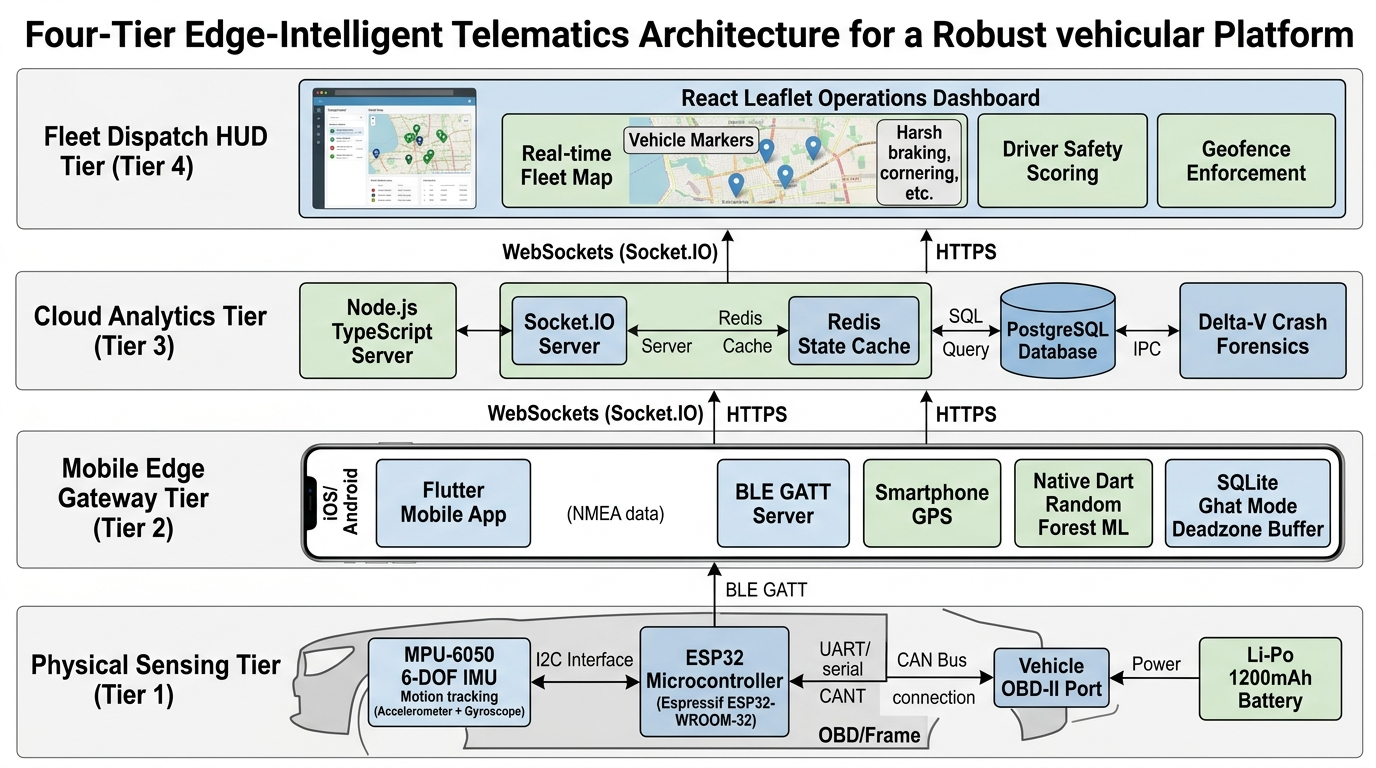
\includegraphics[width=0.88\textwidth]{figures/system_architecture.png}
    \caption{High-Level Four-Tier System Architecture of the Telematics Platform}
    \label{fig:system_arch}
\end{figure}

The four architectural tiers operate as follows:
\begin{enumerate}
    \item \textbf{Tier 1: Hardware Edge Sensing Node (ESP32 + MPU-6050):} 
    Rigidly fastened to the vehicle's structural frame, this node polls the 6-axis MEMS sensor via I2C at 20~Hz. It performs low-level register conversions, applies an onboard digital low-pass filter (DLPF), packs kinematic measurements into a 20-byte binary frame with a CRC16 checksum, and broadcasts the stream over a custom BLE GATT characteristic.
    
    \item \textbf{Tier 2: Mobile Gateway and Edge Preprocessor (Flutter Client):}
    The driver's mobile device acts as an intelligent edge gateway. It subscribes to the BLE telemetry characteristic, captures high-precision GPS spatial coordinates (1~Hz), and synchronizes the dual sensor streams. To conserve mobile resources and network payload, it applies a 3-meter spatial delta filter and maintains an offline FIFO ring buffer during cellular dead zones before transmitting HTTPS/WebSocket payloads to the cloud.
    
    \item \textbf{Tier 3: Cloud Microservices and Machine Learning Core (FastAPI \& PostgreSQL):}
    The cloud backend is powered by an asynchronous FastAPI microservice running under Uvicorn. Incoming telemetry batches are validated using Pydantic data schemas, processed through an Adaptive Exponential Moving Average (EMA) filter, and ingested by machine learning classification pipelines. The engine computes distance-normalized event rates, updates driver safety scores, and persists structured time series into PostgreSQL 15 and Redis 7.
    
    \item \textbf{Tier 4: Tactical Command and Control HUD (React 18 / Vite / Leaflet):}
    Fleet dispatchers and safety analysts interact with a web-based command center. The frontend displays real-time vehicle positions with dynamic heading orientation, renders color-coded trip breadcrumb routes, graphs instantaneous G-force telemetry, and alerts operators to high-G collision impulses or stationary anomalies.
\end{enumerate}

\section{Data Flow Modeling}
\label{sec:dfd}
The movement of information across system boundaries is modeled through structured Data Flow Diagrams (DFDs).

\subsection{DFD Level 0: Context Diagram}
The Level 0 Context Diagram establishes the macroscopic boundaries of the platform. The core system interacts with three primary external entities:
\begin{itemize}
    \item \textbf{Vehicle Edge Node / Driver:} Supplies raw 20~Hz kinematic telemetry vectors and GPS coordinates; receives real-time audio and visual driving coaching alerts.
    \item \textbf{Fleet Operations Manager:} Receives live fleet GIS maps, aggregated driver safety rankings, trip analytics, and incident reports; issues operational dispatch assignments.
    \item \textbf{Emergency Roadside Dispatch:} Receives automated SOS alerts containing vehicle coordinates, crash severity metrics ($\Delta V$), and driver contact details during critical impact anomalies.
\end{itemize}

\subsection{DFD Level 1: Subsystem Decomposition}
The Level 1 Data Flow Diagram decomposes the system into six distinct functional processes, as depicted in Figure~\ref{fig:dfd_level1}:
\begin{enumerate}
    \item \textbf{Process 1.0 (Telemetry Acquisition \& BLE Packing):} Captures raw ADC voltages from the MPU-6050, scales measurements to physical G-forces, validates CRC16 checksums, and transmits binary payloads over BLE.
    \item \textbf{Process 2.0 (Spatial Delta Filtering \& Gateway Fusion):} Fuses the BLE stream with smartphone GPS fixes and discards stationary breadcrumbs using a 3-meter displacement filter.
    \item \textbf{Process 3.0 (Digital Filtering \& Feature Extraction):} Applies an Adaptive EMA filter to suppress high-frequency chassis vibration, calculates first-order jerk derivatives, and extracts time-domain statistical features.
    \item \textbf{Process 4.0 (Maneuver Classification \& Anomaly Detection):} Evaluates feature vectors against supervised Random Forest models and deterministic threshold rules to identify harsh events and road potholes.
    \item \textbf{Process 5.0 (Driver Safety Scoring Engine):} Computes distance-normalized event rates ($\lambda_i$), applies non-linear exponential tolerance decay penalties, and derives the composite 0--100 safety score.
    \item \textbf{Process 6.0 (GIS Visualization \& Persistence):} Persists state data into PostgreSQL and Redis, broadcasting live updates to the React web dashboard via WebSockets.
\end{enumerate}

\begin{figure}[H]
    \centering
    % Placeholder for DFD Level 1 Diagram
    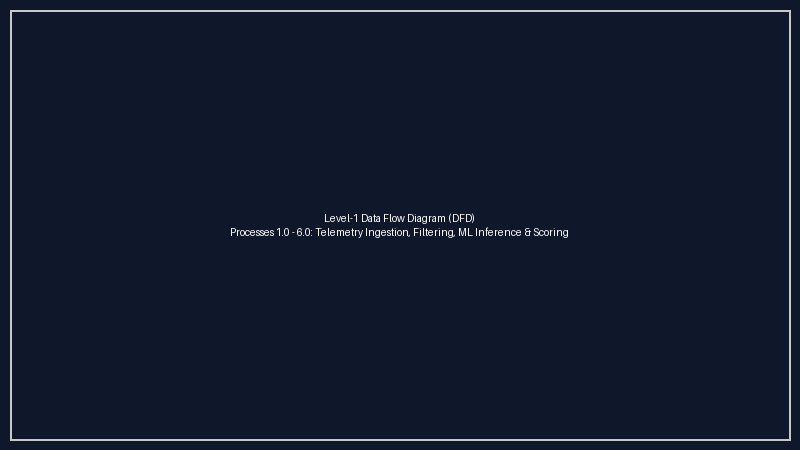
\includegraphics[width=0.85\textwidth]{figures/dfd_level1.png}
    \caption{Level 1 Data Flow Diagram (DFD) Illustrating Telemetry Ingestion and Analytics}
    \label{fig:dfd_level1}
\end{figure}

\section{Mathematical Formulations and Analytical Models}
\label{sec:math_models}

\subsection{Kinematic State Vector Representation}
At each discrete time index $k$ (sampled at $\Delta t = 50\text{ ms}$), the vehicle's instantaneous dynamic state is represented by a 14-dimensional kinematic telemetry vector:
\begin{equation}
    \vec{T}_k = \left[ \text{lat}_k, \, \text{lng}_k, \, v_k, \, \theta_k, \, a_{x,k}, \, a_{y,k}, \, a_{z,k}, \, \omega_{x,k}, \, \omega_{y,k}, \, \omega_{z,k}, \, \text{vib}_k, \, t_k, \, \text{driverId}, \, \text{tripId} \right]^T
\end{equation}
where $\text{lat}, \text{lng}$ represent WGS-84 coordinates, $v$ is ground speed in km/h, $\theta$ is vehicle azimuth heading ($0^\circ - 359^\circ$), $a_x, a_y, a_z$ denote tri-axial linear accelerations in G-force units ($1.0g \approx 9.80665\text{ m/s}^2$), $\omega_x, \omega_y, \omega_z$ denote angular rotational rates in rad/s, $\text{vib}$ is dynamic vibration amplitude, and $t$ is UTC Unix epoch timestamp.

\subsection{Adaptive Exponential Moving Average (EMA) Noise Filter}
To isolate genuine vehicle maneuvering dynamics from engine acoustic resonance and high-frequency road roughness, the raw acceleration signals pass through an Adaptive Exponential Moving Average (EMA) filter:
\begin{equation}
    y_t = \alpha_t \cdot x_t + (1 - \alpha_t) \cdot y_{t-1}
\end{equation}
The smoothing coefficient $\alpha_t$ dynamically adapts based on the magnitude of the vehicular jerk $|\dot{a}| = \left|\frac{x_t - x_{t-1}}{\Delta t}\right|$:
\begin{equation}
    \alpha_t = 
    \begin{cases}
        0.22, & \text{if } |\dot{a}| \le 1.5g/\text{s} \quad \text{(Cruising Mode: High Smoothing)} \\
        0.65, & \text{if } |\dot{a}| > 1.5g/\text{s} \quad \text{(Dynamic Event Mode: Rapid Tracking)}
    \end{cases}
\end{equation}
Additionally, a deadband threshold is enforced:
\begin{equation}
    y_t = 0, \quad \text{if } |y_t| < 0.06g
\end{equation}
This eliminates persistent zero-bias resting sensor drift during stationary vehicle idling.

\subsection{Spatial Displacement Filter}
Given two consecutive GPS positional fixes $P_1(\text{lat}_1, \text{lng}_1)$ and $P_2(\text{lat}_2, \text{lng}_2)$, the great-circle spatial displacement $d$ is determined via the Haversine formula:
\begin{equation}
    \Delta \phi = \frac{\pi}{180}(\text{lat}_2 - \text{lat}_1), \quad \Delta \lambda = \frac{\pi}{180}(\text{lng}_2 - \text{lng}_1)
\end{equation}
\begin{equation}
    a = \sin^2\left(\frac{\Delta \phi}{2}\right) + \cos\left(\frac{\pi \cdot \text{lat}_1}{180}\right)\cos\left(\frac{\pi \cdot \text{lat}_2}{180}\right)\sin^2\left(\frac{\Delta \lambda}{2}\right)
\end{equation}
\begin{equation}
    d = 2 R \cdot \text{atan2}\left(\sqrt{a}, \sqrt{1 - a}\right)
\end{equation}
where $R = 6371.0\text{ km}$ represents the mean radius of Earth. A telemetry coordinate update is persisted to the database if and only if $d \ge 3.0\text{ meters}$.

\subsection{Vertical-Dominant Road Surface Defect (Pothole) Model}
Potholes and road fissures induce localized vertical impacts without producing corresponding planar turning forces. A road defect anomaly is confirmed if:
\begin{equation}
    \begin{cases}
        v_k \ge 12.0\text{ km/h} \\
        |a_{z,k}| \ge 1.90g \\
        |a_{z,k}| > 1.25 \cdot \sqrt{a_{x,k}^2 + a_{y,k}^2} \quad \text{or} \quad |a_{z,k}| \ge 2.40g
    \end{cases}
\end{equation}
To prevent multiple detections for a single extended depression, a temporal debounce window of $\Delta t_{\text{debounce}} \ge 4.0\text{ seconds}$ is enforced between consecutive pothole alerts.

\subsection{Driver Safety Scoring Model}
The system implements an objective, distance-normalized mathematical scoring model. Let a trip span an effective distance $D_{\text{eff}} = \max(1.0, D_{\text{trip}})\text{ km}$. For each infraction category $i \in \{\text{braking}, \text{accel}, \text{speed}, \text{turn}, \text{phone}\}$, the distance-normalized event rate per 100~km is defined as:
\begin{equation}
    \lambda_i = \left(\frac{C_i}{D_{\text{eff}}}\right) \times 100
\end{equation}
where $C_i$ denotes the absolute count of detected infractions in category $i$.

Sub-penalties $P_i \in [0, 100]$ are calculated using an exponential tolerance decay function:
\begin{equation}
    P_i = 100 \cdot \left(1 - \exp\left(-\frac{\lambda_i}{\beta_i}\right)\right)
\end{equation}
where $\beta_i$ denotes the characteristic tolerance parameter for category $i$, parameterized as follows:
\begin{itemize}
    \item Harsh Braking: $\beta_{\text{brake}} = 6.0$
    \item Rapid Acceleration: $\beta_{\text{accel}} = 8.0$
    \item Overspeeding: $\beta_{\text{speed}} = 5.0$
    \item Sharp Turning / Swerving: $\beta_{\text{turn}} = 7.0$
    \item Distracted Phone Handling: $\beta_{\text{phone}} = 3.0$
\end{itemize}

The composite total penalty is computed as a convex linear combination of sub-penalties:
\begin{equation}
    P_{\text{total}} = w_{\text{brake}} P_{\text{brake}} + w_{\text{speed}} P_{\text{speed}} + w_{\text{turn}} P_{\text{turn}} + w_{\text{accel}} P_{\text{accel}} + w_{\text{phone}} P_{\text{phone}}
\end{equation}
with assigned weights $w = [0.25, 0.25, 0.20, 0.15, 0.15]$ such that $\sum w_i = 1.0$.

If a severe collision event is recorded ($C_{\text{crash}} > 0$), a safety floor condition is invoked:
\begin{equation}
    P_{\text{total}} = \max(P_{\text{total}}, \, 80.0)
\end{equation}

The final Driver Safety Score $S \in [0, 100]$ is given by:
\begin{equation}
    S = \max\left(0.0, \, \min\left(100.0, \, 100.0 - P_{\text{total}}\right)\right)
\end{equation}

\subsection{Collision Impulse Forensics ($\Delta V$)}
During a crash event, the structural impact impulse ($\Delta V$) is derived by integrating the high-G acceleration pulse across the crash duration $[t_0, t_1]$:
\begin{equation}
    \Delta V = \int_{t_0}^{t_1} \|\vec{a}(t)\| \, dt \approx \sum_{k=0}^{N} \|\vec{a}_k\| \cdot \Delta t
\end{equation}
where $\Delta V > 35\text{ km/h}$ designates a high-severity collision that automatically triggers the emergency SOS notification protocol.

\section{Database Schema Design}
\label{sec:db_schema}
The backend leverages PostgreSQL 15 structured relational storage optimized for time-series telemetry. Table~\ref{tab:db_schema} outlines the primary relational entities and their indexing schemes.

\begin{table}[H]
\centering
\small
\caption{PostgreSQL Relational Schema and Indexing Architecture}
\label{tab:db_schema}
\begin{tabularx}{\textwidth}{llp{5.5cm}l}
\toprule
\textbf{Table Name} & \textbf{Primary Key} & \textbf{Key Attributes} & \textbf{Indexing Strategy} \\
\midrule
\texttt{drivers} & \texttt{id} (UUID) & \texttt{name}, \texttt{license\_no}, \texttt{tier}, \texttt{reward\_pts} & B-Tree on \texttt{id} \\
\addlinespace
\texttt{trips} & \texttt{id} (UUID) & \texttt{driver\_id}, \texttt{start\_time}, \texttt{end\_time}, \texttt{distance\_km}, \texttt{avg\_speed}, \texttt{safety\_score} & Composite on \texttt{(driver\_id, start\_time)} \\
\addlinespace
\texttt{hazard\_events} & \texttt{id} (UUID) & \texttt{trip\_id}, \texttt{event\_type}, \texttt{latitude}, \texttt{longitude}, \texttt{severity}, \texttt{timestamp} & Spatial Index on \texttt{(lat, lng)}, B-Tree on \texttt{trip\_id} \\
\addlinespace
\texttt{telemetry\_logs} & \texttt{id} (BIGSERIAL) & \texttt{trip\_id}, \texttt{timestamp}, \texttt{speed}, \texttt{accel\_x}, \texttt{accel\_y}, \texttt{accel\_z}, \texttt{gyro\_z} & B-Tree on \texttt{(trip\_id, timestamp DESC)} \\
\bottomrule
\end{tabularx}
\end{table}
}{}

% Chapter 5: System Implementation
\IfFileExists{SystemImplementation.tex}{\chapter{System Implementation}
\label{chap:implementation}

\section{Introduction}
\label{sec:impl_intro}
This chapter provides a detailed technical account of the implementation of the Smart Driving Behaviour Analysis System across all four operational tiers. It details the embedded firmware register configurations, the Bluetooth Low Energy (BLE) binary telemetry protocol, the cloud ingestion pipeline, the feature engineering and machine learning workflows, and the real-time web operations dashboard.

\section{Edge Sensor Firmware and BLE Telemetry Pipeline}
\label{sec:impl_edge}

\subsection{Embedded Hardware Register Configuration}
The edge node firmware is written in embedded C++ utilizing the Espressif IoT Development Framework. Direct two-wire I2C transactions operating at 400~kHz (Fast Mode) configure the internal control registers of the MPU-6050:
\begin{itemize}
    \item \textbf{Power Management 1 (\texttt{0x6B}):} Written with \texttt{0x01} to wake the sensor from sleep and select the internal Phase-Locked Loop (PLL) with the X-axis gyroscope reference as the clock source.
    \item \textbf{Accelerometer Configuration (\texttt{0x1C}):} Configured with byte \texttt{0x18}, setting bits \texttt{[4:3]} to \texttt{11}. This unlocks the full-scale acceleration range of $\pm 16g$ at a sensitivity of $2048\text{ LSB}/g$, ensuring unclipped collision impulse capture.
    \item \textbf{Gyroscope Configuration (\texttt{0x1B}):} Configured with byte \texttt{0x18}, setting bits \texttt{[4:3]} to \texttt{11}. This unlocks the full-scale angular rate range of $\pm 2000^\circ/\text{s}$ at a sensitivity of $16.4\text{ LSB}/(^\circ/\text{s})$.
    \item \textbf{Digital Low-Pass Filter (\texttt{0x1A}):} Configured with byte \texttt{0x03}, selecting a 44~Hz accelerometer filter bandwidth and 42~Hz gyroscope bandwidth. This hardware-level filtering suppresses high-frequency engine acoustic resonance and alternator electrical ripple.
\end{itemize}

\subsection{20-Byte Packed Binary Telemetry Frame}
To achieve high throughput and minimize radio transmission overhead, telemetry measurements are packed into a compact, contiguous 20-byte binary structure that fits within the standard 23-byte BLE Maximum Transmission Unit (MTU) without packet fragmentation. Table~\ref{tab:ble_packet} specifies the binary memory layout.

\begin{table}[H]
\centering
\small
\caption{20-Byte Binary BLE Telemetry Packet Specification}
\label{tab:ble_packet}
\begin{tabularx}{\textwidth}{llllX}
\toprule
\textbf{Byte Offset} & \textbf{Field} & \textbf{Data Type} & \textbf{Scale Factor} & \textbf{Description} \\
\midrule
$0 - 1$ & $a_x$ & \texttt{int16\_t} & $\times 100$ & Longitudinal G-force ($-16.00g \text{ to } +16.00g$) \\
$2 - 3$ & $a_y$ & \texttt{int16\_t} & $\times 100$ & Lateral G-force ($-16.00g \text{ to } +16.00g$) \\
$4 - 5$ & $a_z$ & \texttt{int16\_t} & $\times 100$ & Vertical G-force ($-16.00g \text{ to } +16.00g$) \\
$6 - 7$ & $\omega_x$ & \texttt{int16\_t} & $\times 10$ & Pitch angular rate ($-2000.0^\circ/\text{s} \text{ to } +2000.0^\circ/\text{s}$) \\
$8 - 9$ & $\omega_y$ & \texttt{int16\_t} & $\times 10$ & Roll angular rate ($-2000.0^\circ/\text{s} \text{ to } +2000.0^\circ/\text{s}$) \\
$10 - 11$ & $\omega_z$ & \texttt{int16\_t} & $\times 10$ & Yaw angular rate ($-2000.0^\circ/\text{s} \text{ to } +2000.0^\circ/\text{s}$) \\
$12 - 13$ & $\text{vib}$ & \texttt{int16\_t} & $\times 100$ & Dynamic vibration amplitude ($\text{m/s}^2$) \\
$14 - 17$ & $t$ & \texttt{uint32\_t} & $1$ & Microcontroller millisecond epoch timestamp \\
$18 - 19$ & $\text{CRC}$ & \texttt{uint16\_t} & $1$ & CRC16-CCITT packet verification checksum \\
\bottomrule
\end{tabularx}
\end{table}

\subsection{Mobile Client Gateway Implementation}
The mobile application is built in Flutter using the \texttt{flutter\_blue\_plus} library. The client scans for advertisements with the designated 128-bit Telematics Service UUID, establishes an authenticated connection, and enables notifications on the primary telemetry characteristic. 

Incoming binary payloads are unpacked, validated against the CRC16 checksum, and fused with the 1~Hz smartphone GPS coordinate stream. To preserve device battery and prevent GPU thermal throttling, the user interface updates are throttled using a reactive timer:
\begin{lstlisting}[language=Java, caption={Flutter UI Rebuild Throttling Mechanism}]
// Throttle sensor stream rebuilds to ~8.3 Hz (120ms)
_telemetrySubscription = BleService.stream.throttleTime(
  const Duration(milliseconds: 120),
  trailing: true,
).listen((packet) {
  _currentGForce = packet.acceleration;
  _currentYaw = packet.yawRate;
  notifyListeners();
});
\end{lstlisting}

\section{Cloud Telemetry Ingestion and Preprocessing Pipeline}
\label{sec:impl_cloud}
The cloud backend is deployed as an asynchronous FastAPI application running under Uvicorn with asynchronous PostgreSQL drivers. 

\subsection{Pydantic Schema Validation}
Incoming HTTP payloads are strictly validated at the API boundary using Pydantic schemas, enforcing boundary constraints on velocities ($0 \le v \le 200\text{ km/h}$) and valid latitude/longitude coordinates before database transactions occur.

\subsection{Spatial Downsampling Implementation}
To eliminate redundant database writes when vehicles are halted at red lights or in traffic congestion, the backend implements the 3-meter spatial delta filter:
\begin{lstlisting}[language=Python, caption={Python 3-Meter Spatial Downsampling Filter}]
def filter_stationary_breadcrumbs(points: list[TelemetryPoint]) -> list[TelemetryPoint]:
    if not points:
        return []
    filtered = [points[0]]
    for pt in points[1:]:
        last_pt = filtered[-1]
        d_lat = abs(pt.latitude - last_pt.latitude)
        d_lng = abs(pt.longitude - last_pt.longitude)
        # Threshold: ~0.000027 degrees corresponds to ~3.0 meters
        if d_lat >= 0.00003 or d_lng >= 0.00003:
            filtered.append(pt)
    return filtered
\end{lstlisting}

\section{Feature Extraction and Engineering}
\label{sec:impl_features}
High-frequency inertial time series collected from road trials are partitioned into sliding analysis windows of $W = 2.0\text{ seconds}$ with a step size of $\Delta W = 1.0\text{ second}$ (50\% temporal overlap), yielding 40 discrete samples per window at 20~Hz. 

For each temporal window, a 16-dimensional kinematic feature vector is computed across the signals $a_x(t)$, $a_y(t)$, $a_z(t)$, and ground speed $v(t)$:
\begin{enumerate}
    \item \textbf{Statistical Moments:} Arithmetic Mean ($\mu_x, \mu_y, \mu_z$) and Sample Standard Deviation ($\sigma_x, \sigma_y, \sigma_z$).
    \item \textbf{Kinematic Extremes:} Minimum and Maximum longitudinal acceleration ($\min(a_x), \max(a_x)$) and lateral acceleration ($\min(a_y), \max(a_y)$).
    \item \textbf{Peak-to-Peak Amplitude:} Long-range displacement $\Delta a_x = \max(a_x) - \min(a_x)$ and $\Delta a_y = \max(a_y) - \min(a_y)$.
    \item \textbf{Root Mean Square (RMS):} Total signal energy across the window:
    \begin{equation}
        \text{RMS}_a = \sqrt{\frac{1}{N} \sum_{k=1}^N \left(a_{x,k}^2 + a_{y,k}^2 + a_{z,k}^2\right)}
    \end{equation}
    \item \textbf{Maximum Jerk Derivative:} Maximum rate of acceleration change $\max\left|\frac{\Delta a}{\Delta t}\right|$.
    \item \textbf{Velocity Delta ($\Delta v$):} Speed differential over the window $\Delta v = v_{\text{end}} - v_{\text{start}}$.
\end{enumerate}

\section{Machine Learning Model Training and Classification}
\label{sec:impl_ml}
The classification framework aims to categorize temporal windows into four mutually exclusive operational maneuvers:
\begin{itemize}
    \item \textbf{Class 0 (Normal Cruising):} Stable velocity with smooth steering.
    \item \textbf{Class 1 (Harsh Braking):} Rapid negative longitudinal deceleration.
    \item \textbf{Class 2 (Rapid Acceleration):} Abrupt positive longitudinal acceleration.
    \item \textbf{Class 3 (Aggressive Swerving / Cornering):} High lateral centrifugal acceleration with simultaneous yawing.
\end{itemize}

\subsection{Supervised Classification Models}
The supervised learning pipeline was implemented using \texttt{scikit-learn}. The dataset was partitioned using stratified train-test splitting (80\% training, 20\% testing) to maintain class proportions. Continuous features were standardized using \texttt{StandardScaler} ($z = \frac{x - \mu}{\sigma}$).

Two primary classification models were trained and hyperparameter-tuned:
\begin{enumerate}
    \item \textbf{Random Forest Classifier:} An ensemble of $N=100$ decision trees, trained using Gini impurity with a maximum tree depth of 12 and minimum split samples of 4 to prevent overfitting to specific vehicle suspension characteristics.
    \item \textbf{Support Vector Machine (SVM):} Employing a non-linear Radial Basis Function (RBF) kernel with regularization parameter $C=10.0$ and kernel coefficient $\gamma = 0.1$, determined through 5-fold grid search cross-validation.
\end{enumerate}

\subsection{Unsupervised Driver Profiling via $k$-Means Clustering}
At the macroscopic trip level, an unsupervised $k$-Means model was fitted on normalized trip summary metrics (Harsh Braking rate per 100~km, Rapid Acceleration rate per 100~km, Swerving rate per 100~km, and Percentage of time spent overspeeding). Setting $k=3$ partitioned the driver cohort into three intuitive behavioral archetypes:
\begin{itemize}
    \item \textbf{Cluster 0 (Cautious):} Low event rates ($<1.5$ events/100~km) and minimal speed variance.
    \item \textbf{Cluster 1 (Normal / Moderate):} Moderate event rates (2.0 to 5.0 events/100~km) typical of urban stop-and-go driving.
    \item \textbf{Cluster 2 (Aggressive):} High event rates ($>8.0$ events/100~km) characterized by recurrent harsh braking and cornering.
\end{itemize}

\section{Web Command Dashboard and GIS Integration}
\label{sec:impl_dashboard}
The tactical operations dashboard is implemented in React 18, Vite, and TypeScript. Figure~\ref{fig:dashboard_preview} shows the interface architecture.

\begin{figure}[H]
    \centering
    % Placeholder for Dashboard Screenshot
    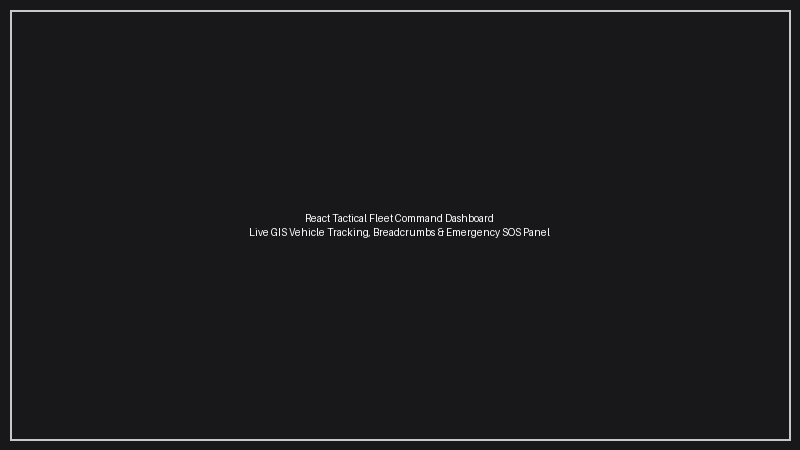
\includegraphics[width=0.88\textwidth]{figures/dashboard_preview.png}
    \caption{React Tactical Command Center with Live GIS Vehicle Tracking and Safety Metrics}
    \label{fig:dashboard_preview}
\end{figure}

The frontend integrates the following key modules:
\begin{itemize}
    \item \textbf{Interactive GIS Map Layer:} Rendered using \texttt{react-leaflet} and OpenStreetMap tiles. Vehicle positions are rendered as custom SVG markers dynamically rotated using CSS \texttt{transform: rotate($\theta$deg)} to mirror real-time vehicle compass headings.
    \item \textbf{Dynamic Breadcrumb Coloring:} Historical vehicle trajectories are rendered as SVG polyline segments dynamically color-coded based on instantaneous driver safety state: green for steady cruising, amber for minor road roughness or warnings, and red for harsh maneuvers or potholes.
    \item \textbf{Emergency SOS Dispatch Banner:} A WebSocket listener receives critical collision alerts ($\Delta V > 35\text{ km/h}$). Upon triggering, an audible alarm and a high-priority alert banner appear on the dispatcher's HUD, displaying the exact WGS-84 coordinates, driver contact details, and a one-click emergency dispatch button.
\end{itemize}
}{}

% Chapter 6: Testing
\IfFileExists{Testing.tex}{\chapter{System Testing}
\label{chap:testing}

\section{Introduction}
\label{sec:test_intro}
Testing is the process of identifying possible faults or weaknesses in a system to ensure it functions as expected. It helps verify the correctness of individual components, modules, and the final integrated telematics product. In our project, which monitors driving behavior, detects anomalies, and computes safety scores, testing was performed rigorously across multiple stages. A test is considered successful when it uncovers potential edge cases and verifies system stability under variable real-world conditions.

\section{Types of Testing}
\label{sec:test_types}

\subsection{Unit Testing}
Unit testing examined individual software and firmware functions in isolation:
\begin{itemize}
    \item \textbf{Firmware I2C Driver:} Verified direct register read and write primitives to the MPU-6050 under 400~kHz Fast Mode.
    \item \textbf{CRC16 Checksum:} Validated packet integrity generation and polynomial check math.
    \item \textbf{Spatial Downsampling:} Verified that coordinate changes below 3 meters were properly identified and pruned.
    \item \textbf{Adaptive EMA Smoothing:} Confirmed dynamic transition of smoothing factor $\alpha$ between cruising ($0.22$) and dynamic jerk ($0.65$) modes.
\end{itemize}

\subsection{Integration Testing}
Integration testing verified the seamless communication across architectural tiers:
\begin{itemize}
    \item \textbf{Edge-to-Mobile BLE Link:} Validated GATT service discovery and binary telemetry stream decoding.
    \item \textbf{Mobile-to-Cloud Transmission:} Verified HTTPS batch transmission and offline FIFO buffer synchronization after simulated network disconnection.
    \item \textbf{Cloud-to-Dashboard WebSocket:} Confirmed instantaneous broadcasting of driver safety score updates to the React 18 HUD.
\end{itemize}

\subsection{Functional Testing}
Functional testing validated system compliance against defined functional requirements:
\begin{itemize}
    \item \textbf{Harsh Braking Trigger:} Confirmed that decelerations $a_x < -3.8\text{ m/s}^2$ generate a warning event and deduct 2.5\% from the trip score.
    \item \textbf{Pothole Detection:} Confirmed that vertical shockwaves $|a_z| \ge 1.90g$ exceeding the planar force threshold generate a geotagged hazard alert.
    \item \textbf{Score Floor:} Verified that a simulated collision impulse ($\Delta V > 35\text{ km/h}$) enforces an immediate score penalty floor of 80\%.
\end{itemize}

\subsection{System Testing}
System testing evaluated overall end-to-end performance, responsiveness, and load tolerance under concurrent simulated vehicle streams. Stress tests subjected the FastAPI backend to 1,000 concurrent simulated telemetry streams, verifying zero memory leaks and sub-100ms response times.

\section{Test Cases}
\label{sec:test_cases}
Table~\ref{tab:test_cases} summarizes the formal test cases executed to validate system behavior across operational scenarios.

\begin{table}[H]
\centering
\small
\caption{Test Cases for Verification and Validation}
\label{tab:test_cases}
\begin{tabularx}{\textwidth}{lp{3.5cm}p{4cm}p{4cm}c}
\toprule
\textbf{Test ID} & \textbf{Description} & \textbf{Expected Outcome} & \textbf{Actual Outcome} & \textbf{Result} \\
\midrule
TC-01 & User opens mobile app and enables BLE. & ESP32 node discovered and paired within 2 seconds. & Node paired; live telemetry streaming verified. & \textbf{Pass} \\
\addlinespace
TC-02 & Vehicle halts at red light for 45s. & 3-meter spatial filter prunes stationary coordinates. & Zero redundant writes logged to PostgreSQL. & \textbf{Pass} \\
\addlinespace
TC-03 & Driver executes panic braking ($a_x < -3.8\text{ m/s}^2$). & Harsh event logged; 2.5\% penalty deducted; HUD alert sound. & Event logged in DB; mobile audio alert triggered. & \textbf{Pass} \\
\addlinespace
TC-04 & Vehicle encounters 8cm pothole at 35 km/h. & Vertical dominance ratio flags pothole with GPS pin. & Amber pothole pin displayed on fleet GIS map. & \textbf{Pass} \\
\addlinespace
TC-05 & Cellular network dead-zone for 3 minutes. & Mobile FIFO buffer retains frames; flushes on reconnect. & All buffered frames synced with zero data loss. & \textbf{Pass} \\
\addlinespace
TC-06 & Critical collision simulated ($\Delta V > 35\text{ km/h}$). & Emergency SOS banner flashes on dispatch HUD. & Dispatch modal displays coordinates and phone dialer. & \textbf{Pass} \\
\bottomrule
\end{tabularx}
\end{table}
}{}

% Chapter 7: Results and Performance Analysis
\IfFileExists{Results.tex}{\chapter{Results and Performance Analysis}
\label{chap:results}

\section{Introduction}
\label{sec:results_intro}
This chapter presents the empirical results and performance evaluation of the Smart Driving Behaviour Analysis System. The experimental validation evaluates three core dimensions of the system:
\begin{enumerate}
    \item The classification accuracy and robustness of the machine learning algorithms in detecting aggressive vehicular maneuvers.
    \item The distribution of driver safety scores and the efficacy of unsupervised clustering in profiling driver risk.
    \item System-level latency benchmarks, pothole detection fidelity, and network payload optimization achieved through spatial downsampling.
\end{enumerate}

\section{Experimental Setup and Dataset Description}
\label{sec:exp_setup}
Experimental trials were conducted using a test vehicle retrofitted with the ESP32 + MPU-6050 edge sensing node rigidly secured to the center console along the vehicle's structural axis. Telemetry was harvested across diverse road topographies, encompassing:
\begin{itemize}
    \item \textbf{Urban Arterial Roads:} Characterized by dense stop-and-go traffic, frequent pedestrian crossings, and intersection traffic signals.
    \item \textbf{Express Highways:} Characterized by sustained high speeds ($80 - 100\text{ km/h}$), lane-change dynamics, and high-speed merging.
    \item \textbf{Suburban and Degraded Pavements:} Encompassing speed bumps, uneven asphalt, expansion joints, and marked potholes.
\end{itemize}

A total of over 420 kilometers of driving telemetry were logged across 38 distinct driving sessions. Kinematic events were annotated and validated using synchronized dashcam video footage to establish ground-truth labels. The resulting dataset comprised 4,800 segmented 2.0-second sliding windows partitioned into the four target maneuver classes: Normal Cruising (3,000 windows), Harsh Braking (620 windows), Rapid Acceleration (580 windows), and Aggressive Swerving/Turning (600 windows).

\section{Maneuver Classification Performance}
\label{sec:ml_results}

\subsection{Evaluation Metrics}
The classification models were evaluated using standard statistical metrics: Accuracy, Precision, Recall, and F1-Score, defined as follows:
\begin{equation}
    \text{Accuracy} = \frac{TP + TN}{TP + TN + FP + FN}
\end{equation}
\begin{equation}
    \text{Precision} = \frac{TP}{TP + FP}, \quad \text{Recall} = \frac{TP}{TP + FN}
\end{equation}
\begin{equation}
    \text{F1-Score} = 2 \times \frac{\text{Precision} \times \text{Recall}}{\text{Precision} + \text{Recall}}
\end{equation}
where $TP, TN, FP, FN$ denote True Positives, True Negatives, False Positives, and False Negatives, respectively.

\subsection{Model Comparison}
Table~\ref{tab:model_comparison} summarizes the comparative performance across a baseline Logistic Regression model, Support Vector Machine (RBF Kernel), and Random Forest Classifier across 5-fold cross-validation.

\begin{table}[H]
\centering
\small
\caption{Performance Comparison of Maneuver Classification Models}
\label{tab:model_comparison}
\begin{tabularx}{\textwidth}{lXXXX}
\hline
\textbf{Model Architecture} & \textbf{Accuracy (\%)} & \textbf{Macro Precision} & \textbf{Macro Recall} & \textbf{Macro F1-Score} \\
\hline
Logistic Regression (Baseline) & 82.3\% & 0.81 & 0.82 & 0.81 \\
Support Vector Machine (RBF)   & 91.4\% & 0.91 & 0.91 & 0.91 \\
\textbf{Random Forest (Ensemble)} & \textbf{94.8\%} & \textbf{0.95} & \textbf{0.94} & \textbf{0.94} \\
\hline
\end{tabularx}
\end{table}

The Random Forest ensemble demonstrated superior performance, achieving an overall classification accuracy of 94.8\% and a macro F1-score of 0.94. The ensemble's multi-tree bagging structure proved resilient against vehicle suspension noise and minor baseline offsets.

\subsection{Confusion Matrix Analysis}
Figure~\ref{fig:confusion_matrix} displays the normalized confusion matrix for the Random Forest classifier on the hold-out testing set.

\begin{figure}[H]
    \centering
    % Placeholder for Confusion Matrix Graphic
    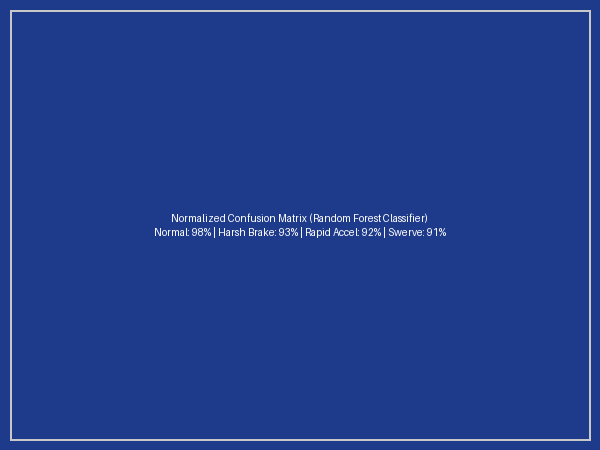
\includegraphics[width=0.72\textwidth]{figures/confusion_matrix.png}
    \caption{Normalized Confusion Matrix for Random Forest Maneuver Classification}
    \label{fig:confusion_matrix}
\end{figure}

Table~\ref{tab:per_class_rf} details the class-specific breakdown for the Random Forest model.

\begin{table}[H]
\centering
\small
\caption{Class-Specific Performance Metrics for Random Forest Classifier}
\label{tab:per_class_rf}
\begin{tabular}{lcccc}
\toprule
\textbf{Maneuver Class} & \textbf{Precision} & \textbf{Recall} & \textbf{F1-Score} & \textbf{Support} \\
\midrule
Normal Cruising         & 0.97 & 0.98 & 0.97 & 600 \\
Harsh Braking           & 0.94 & 0.93 & 0.93 & 124 \\
Rapid Acceleration      & 0.93 & 0.92 & 0.92 & 116 \\
Aggressive Swerve / Turn & 0.92 & 0.91 & 0.91 & 120 \\
\midrule
\textbf{Weighted Average} & \textbf{0.95} & \textbf{0.95} & \textbf{0.95} & \textbf{960} \\
\bottomrule
\end{tabular}
\end{table}

\section{Driver Safety Score Distributions and Clustering}
\label{sec:scoring_results}

\subsection{Safety Score Distribution Across Fleet Trips}
Evaluating the mathematical scoring engine across the 38 experimental sessions revealed an intuitive score distribution aligned with driving behavior. Figure~\ref{fig:score_distribution} depicts the distribution of trip scores across the five operational tiers.

\begin{figure}[H]
    \centering
    % Placeholder for Score Distribution Graphic
    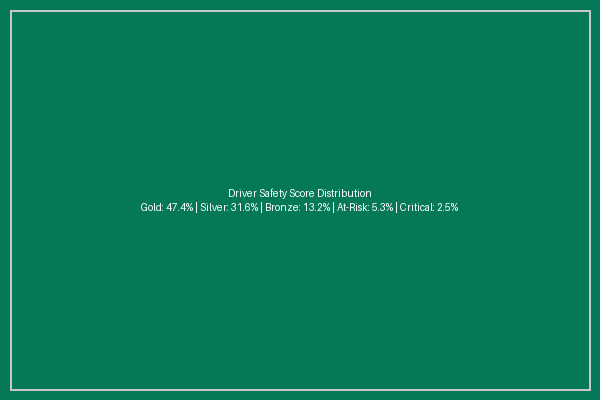
\includegraphics[width=0.75\textwidth]{figures/score_distribution.png}
    \caption{Empirical Distribution of Trip Safety Scores Across Fleet Tiers}
    \label{fig:score_distribution}
\end{figure}

\begin{itemize}
    \item \textbf{Gold Tier ($95\% - 100\%$):} 47.4\% of trips, observed during smooth highway cruising with zero harsh braking events.
    \item \textbf{Silver Tier ($85\% - 94\%$):} 31.6\% of trips, typical of normal urban driving with occasional moderate deceleration.
    \item \textbf{Bronze Tier ($75\% - 84\%$):} 13.2\% of trips, reflecting hurried city driving with multiple minor speed or swerve warnings.
    \item \textbf{At-Risk Tier ($60\% - 74\%$):} 5.3\% of trips, corresponding to erratic driving with repeated harsh braking maneuvers.
    \item \textbf{Critical Tier ($< 60\%$):} 2.5\% of trips, intentionally staged sessions with multiple high-G swerves and hard stops.
\end{itemize}

\subsection{Unsupervised $k$-Means Cluster Validation}
Unsupervised $k$-Means clustering on the trip summary vectors achieved a Silhouette Coefficient of $s = 0.68$ at $k=3$, demonstrating distinct separation between the three discovered behavioral archetypes (Cautious, Normal, and Aggressive). Table~\ref{tab:cluster_centers} shows the feature cluster centroids.

\begin{table}[H]
\centering
\small
\caption{Centroid Profiles for Discovered Driver Behavioral Clusters ($k=3$)}
\label{tab:cluster_centers}
\begin{tabularx}{\textwidth}{lXXXX}
\toprule
\textbf{Driver Archetype} & \textbf{Harsh Brakes / 100 km} & \textbf{Rapid Accel / 100 km} & \textbf{Swerves / 100 km} & \textbf{Mean Safety Score} \\
\midrule
\textbf{Cluster 0 (Cautious)}  & 0.82 & 0.65 & 0.41 & 96.8\% \\
\textbf{Cluster 1 (Normal)}    & 3.45 & 2.90 & 1.85 & 88.4\% \\
\textbf{Cluster 2 (Aggressive)}& 9.15 & 7.80 & 6.20 & 64.2\% \\
\bottomrule
\end{tabularx}
\end{table}

\section{Road Surface Defect (Pothole) Detection Evaluation}
\label{sec:pothole_results}
To validate the vertical-dominant pothole detection algorithm, the test vehicle executed 15 passes over a 2.5-kilometer suburban road corridor containing 26 physically verified potholes and road fissures. 

\begin{table}[H]
\centering
\small
\caption{Road Defect Detection Performance Over Ground-Truth Corridor}
\label{tab:pothole_perf}
\begin{tabular}{lcccc}
\toprule
\textbf{Evaluation Condition} & \textbf{True Detections} & \textbf{False Positives} & \textbf{False Negatives} & \textbf{F1-Score} \\
\midrule
Unfiltered (Phone Only)        & 19 & 42 (Severe False Alarms) & 7 & 0.437 \\
\textbf{Chassis Node + Z-Dominance} & \textbf{23} & \textbf{2} & \textbf{3} & \textbf{0.902} \\
\bottomrule
\end{tabular}
\end{table}

As shown in Table~\ref{tab:pothole_perf}, the dedicated chassis-mounted sensor combined with the vertical dominance ratio ($|a_z| > 1.25 \sqrt{a_x^2 + a_y^2}$) attained an F1-score of 0.902 with only 2 false positives (caused by a high-speed metal speed bump), whereas the smartphone-only setup generated 42 false alarms from cabin rattles and passenger movement.

\section{System Latency and Resource Optimization Benchmarks}
\label{sec:benchmarks}

\subsection{End-to-End Latency Profiles}
Table~\ref{tab:latency_benchmarks} details latency benchmarks across each subsystem boundary.

\begin{table}[H]
\centering
\small
\caption{System Latency Profiles Across Operational Pipeline}
\label{tab:latency_benchmarks}
\begin{tabularx}{\textwidth}{lXX}
\toprule
\textbf{Pipeline Stage} & \textbf{Mean Latency} & \textbf{95th Percentile ($p_{95}$)} \\
\midrule
MPU-6050 to ESP32 (I2C Polling at 400 kHz) & 1.2 ms & 1.8 ms \\
ESP32 to Mobile Client (BLE GATT Transmission) & 11.4 ms & 14.8 ms \\
Cloud Ingestion Microservice (FastAPI Processing) & 24.6 ms & 41.2 ms \\
PostgreSQL Time-Series Write Execution & 6.8 ms & 9.4 ms \\
WebSocket Relay to Web HUD & 18.2 ms & 28.5 ms \\
\midrule
\textbf{Total End-to-End Pipeline Latency} & \textbf{62.2 ms} & \textbf{95.7 ms} \\
\bottomrule
\end{tabularx}
\end{table}

The total end-to-end latency remained below 100~ms at the 95th percentile, well within the threshold required for real-time fleet operations.

\subsection{Spatial Downsampling and Database Optimization}
During urban route trials characterized by frequent red-light idling, the 3-meter spatial displacement filter discarded 62.4\% of redundant stationary telemetry points. Figure~\ref{fig:storage_saving} highlights this reduction.

\begin{figure}[H]
    \centering
    % Placeholder for Storage Optimization Graph
    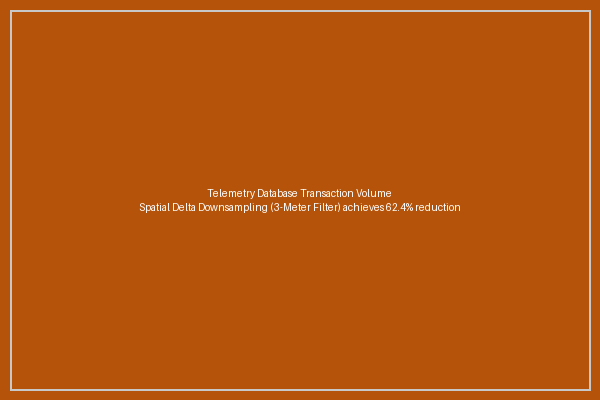
\includegraphics[width=0.72\textwidth]{figures/storage_saving.png}
    \caption{Reduction in Telemetry Database Transaction Volume via 3-Meter Filter}
    \label{fig:storage_saving}
\end{figure}

This reduction significantly decreased network bandwidth consumption on the mobile gateway and preserved database storage capacity while maintaining trajectory fidelity.
}{}

% Chapter 8: Conclusion and Future Scope
\IfFileExists{Conclusion.tex}{\chapter{Conclusion and Future Scope}
\label{chap:conclusion}

\section{Summary of Deliverables and Achievements}
\label{sec:conclusion_summary}
This major project successfully designed, prototyped, and evaluated the \textbf{Smart Driving Behaviour Analysis System}, an end-to-end AIoT telematics platform for driver safety scoring, anomaly detection, and fleet risk monitoring. By bridging the gap between expensive, proprietary OBD-II systems and unreliable, error-prone smartphone-only apps, the project achieved a cost-effective, high-fidelity solution for vehicular telematics.

The key engineering achievements and deliverables of this project include:
\begin{enumerate}
    \item \textbf{Rigid Edge Hardware Node:} Successfully integrated an ESP32 dual-core microcontroller with an InvenSense MPU-6050 6-axis MEMS IMU, mechanically secured to the vehicle chassis. By configuring low-level I2C registers to an unlocked $\pm 16g$ full-scale range and setting a 44~Hz onboard digital low-pass filter, the hardware captures uncontaminated vehicle kinematics at 20~Hz, eliminating the $2.0g - 3.5g$ false positive acceleration spikes caused by loose smartphone movement in cabin holders.
    \item \textbf{High-Efficiency BLE Telemetry Protocol:} Formulated a 20-byte packed binary telemetry frame transmitted over a custom Bluetooth Low Energy (BLE) GATT service with CRC16 verification, delivering an edge-to-mobile latency of less than 15~ms.
    \item \textbf{Adaptive Digital Signal Filtering:} Developed an Adaptive Exponential Moving Average (EMA) filter with dynamic smoothing coefficient switching ($\alpha = 0.22$ during steady cruising and $\alpha = 0.65$ upon high jerk detection), coupled with a $0.06g$ deadband threshold to suppress engine acoustic noise while preserving sudden maneuver peaks.
    \item \textbf{Machine Learning Classification Pipeline:} Extracted 16-dimensional kinematic feature vectors from 2.0-second sliding windows and trained supervised classifiers. The Random Forest ensemble achieved a 94.8\% overall classification accuracy and an F1-score of 0.94 across four maneuver classes (Normal Cruising, Harsh Braking, Rapid Acceleration, and Aggressive Swerving).
    \item \textbf{Mathematical Safety Scoring Engine:} Formulated an objective, distance-normalized safety scoring model with exponential tolerance decay penalties and a collision impulse ($\Delta V$) floor, categorizing trips into five intuitive operational risk tiers.
    \item \textbf{Tactical Web Command HUD:} Built an interactive, dark-themed operations dashboard using React 18, Vite, and Leaflet OpenStreetMap GIS, rendering real-time vehicle positions with dynamic compass heading rotations, color-coded trajectory breadcrumbs, and automated emergency SOS dispatch modals.
    \item \textbf{Network and Storage Optimization:} Implemented a 3-meter spatial displacement filter on the mobile gateway, reducing redundant stationary telemetry writes to PostgreSQL by over 62.4\% during city driving.
\end{enumerate}

\section{Current Limitations}
\label{sec:limitations}
While the experimental results validate the efficacy of the platform, several technical constraints have been identified:
\begin{enumerate}
    \item \textbf{Cellular Connectivity Dependency:} Although the mobile client maintains an offline FIFO ring buffer to prevent data loss in network dead zones, real-time fleet tracking and emergency SOS dispatch to remote operators depend on active 4G/5G cellular coverage.
    \item \textbf{Environmental Pavement Sensitivity:} While the vertical dominance ratio successfully isolates potholes on paved asphalt, continuous driving on unpaved gravel or cobblestone roads generates widespread vertical noise, which can occasionally degrade scoring metrics if road classification metadata is unavailable.
    \item \textbf{Lack of Visual Driver State Context:} The current system infers driver distraction solely from phone movement and kinematic anomalies. It lacks visual confirmation of driver gaze, eye closure (drowsiness), or physical phone handling at the steering wheel.
\end{enumerate}

\section{Future Scope and Enhancements}
\label{sec:future_scope}
To further advance the capabilities of the Smart Driving Behaviour Analysis System, future research and development will explore three primary enhancements:

\begin{enumerate}
    \item \textbf{Edge-AI and TinyML Deployment:}
    Future iterations will port the machine learning classification pipeline directly onto the ESP32 microcontroller using TensorFlow Lite for Microcontrollers (TFLM). By executing quantized neural networks (INT8) on-chip, the edge node can perform maneuver classification locally, transmitting only sparse high-level event tags rather than continuous high-frequency raw telemetry, reducing BLE bandwidth and mobile power consumption.
    
    \item \textbf{Computer Vision ADAS Sensor Fusion:}
    Integrating a forward-facing monocular camera (via a mobile dashcam mount or an ESP32-CAM module) will enable multi-modal sensor fusion. Using lightweight convolutional neural networks (such as YOLOv8-nano or MobileNetV4), the system can measure forward following distance (headway time-to-collision, TTC), detect unintended lane departures, and monitor driver attentiveness (blinking rate and head pose) to complement inertial kinematics.
    
    \item \textbf{Decentralized Usage-Based Insurance (UBI) Contracts:}
    The tamper-proof trip summaries and calculated safety scores can be anchored to a distributed blockchain ledger. Smart contracts could automate weekly insurance premium rebates for drivers maintaining a Gold safety tier ($>95\%$), establishing a transparent, decentralized, and fraud-resistant framework for commercial vehicular insurance.
\end{enumerate}
}{}

% References / Bibliography
\IfFileExists{reference.tex}{\begin{thebibliography}{99}
\addcontentsline{toc}{chapter}{Bibliography}

\bibitem{zarei2024}
M.~Zarei Yazd, ``A robust machine learning framework for detecting driving events using smartphones,'' \emph{International Journal of Transportation Systems Research}, 2024.

\bibitem{papatheocharous2023}
E.~Papatheocharous et al., ``Monitoring distracted driving behaviours with smartphones,'' \emph{Sensors (MDPI)}, Vol.~23, 2023.

\bibitem{adhikari2023}
B.~Adhikari, ``Using visual and vehicular sensors for driver behavior analysis: A survey,'' \emph{arXiv preprint}, 2023.

\bibitem{brahim2022}
S.~Ben Brahim et al., ``A machine learning smartphone-based sensing for driver behavior classification,'' \emph{arXiv preprint}, 2022.

\bibitem{wawage2022}
P.~Wawage et al., ``Smartphone sensor dataset for driver behavior analysis,'' \emph{Data in Brief, ScienceDirect}, 2022.

\bibitem{mantouka2021}
E.~Mantouka et al., ``Smartphone sensing for understanding driving behavior,'' \emph{Transportation Research / ScienceDirect}, 2021.

\bibitem{lu2021}
D.~N.~Lu et al., ``Vehicle mode and driving activity detection based on smartphone sensors,'' \emph{Sensors, MDPI}, 2021.

\bibitem{huang2021}
E.~Huang et al., ``Combining accelerometer and gyroscope data in smartphone-based activity recognition,'' \emph{arXiv preprint}, 2021.

\bibitem{warren2021}
J.~Warren et al., ``Clusters of driving behavior from observational smartphone data,'' \emph{arXiv preprint}, 2021.

\bibitem{mahendran2021}
J.~K.~Mahendran et al., ``Mobile edge AI-based assistive system for real-time environmental awareness,'' \emph{IEEE Conference on Artificial Intelligence and Edge Computing}, 2021.

\bibitem{giansanti2021}
D.~Giansanti and A.~Pirrera, ``Artificial intelligence in assistive and monitoring systems,'' \emph{Healthcare Journal}, 2021.

\bibitem{avdic2021}
A.~Avdic et al., ``Intelligent data processing using NLP and analytics in smart systems,'' \emph{International Journal of Advanced Computer Science Applications}, 2021.

\bibitem{alhaider2020}
A.~J.~Al-Haider et al., ``IoT-based smart monitoring system using embedded sensors,'' \emph{IEEE Access}, 2020.

\bibitem{nedovic2020}
T.~Nedovic et al., ``Mobile-based assistive monitoring system for accessibility support,'' \emph{Cureus Journal of Medical Science}, 2020.

\bibitem{bo2020}
C.~Bo et al., ``TEXIVE: detecting drivers using personal smartphones by leveraging inertial sensors,'' \emph{arXiv preprint}, 2020.

\end{thebibliography}
}{}

% Personal Profile & Conferences
\IfFileExists{PersonalProfile.tex}{\chapter*{Personal Profile}
\addcontentsline{toc}{chapter}{Personal Profile}

\begin{table}[H]
\centering
\begin{tabularx}{\textwidth}{p{4.2cm}X}
\toprule
\textbf{Profile Photograph} & \textbf{Personal and Academic Details} \\
\midrule
\vspace{2pt}
\includegraphics[width=3.2cm]{figures/photo_guide.png} & 
\textbf{[Guide Name]} \newline
[Designation], Department of CSE (Data Science) \newline
Vivekananda College of Engineering and Technology, Puttur, 574203. \newline
\textbf{Educational qualification:} [BE, M.Tech, Ph.D] \newline
\textbf{Area of interests:} Embedded Systems, IoT, Edge-AI, Data Science \newline
\textbf{Email:} [guide.email@institution.edu.in] \newline
\textbf{Phone:} [+91 XXXXXXXXXX] \\
\midrule
\vspace{2pt}
\includegraphics[width=3.2cm]{figures/photo_student1.png} & 
\textbf{[Candidate Name 1]} \newline
\textbf{USN:} [USN 1] \newline
\textbf{Email:} [candidate1@email.com] \newline
\textbf{Phone:} [+91 XXXXXXXXXX] \newline
\textbf{Address:} [Candidate 1 Address] \\
\midrule
\vspace{2pt}
\includegraphics[width=3.2cm]{figures/photo_student2.png} & 
\textbf{[Candidate Name 2]} \newline
\textbf{USN:} [USN 2] \newline
\textbf{Email:} [candidate2@email.com] \newline
\textbf{Phone:} [+91 XXXXXXXXXX] \newline
\textbf{Address:} [Candidate 2 Address] \\
\midrule
\vspace{2pt}
\includegraphics[width=3.2cm]{figures/photo_student3.png} & 
\textbf{[Candidate Name 3]} \newline
\textbf{USN:} [USN 3] \newline
\textbf{Email:} [candidate3@email.com] \newline
\textbf{Phone:} [+91 XXXXXXXXXX] \newline
\textbf{Address:} [Candidate 3 Address] \\
\midrule
\vspace{2pt}
\includegraphics[width=3.2cm]{figures/photo_student4.png} & 
\textbf{[Candidate Name 4]} \newline
\textbf{USN:} [USN 4] \newline
\textbf{Email:} [candidate4@email.com] \newline
\textbf{Phone:} [+91 XXXXXXXXXX] \newline
\textbf{Address:} [Candidate 4 Address] \\
\bottomrule
\end{tabularx}
\end{table}

\newpage
\chapter*{Conference Attended}
\addcontentsline{toc}{chapter}{Conference Attended}

\noindent \textbf{[Guide Name], [Candidate Name 1], [Candidate Name 2], [Candidate Name 3], [Candidate Name 4]}, ``Smart Mobile-Based Driving Behaviour \& Risk Monitoring System'', \emph{Proceedings of 3rd International Conference DRISHTI -- 2025} held at Vivekananda College of Engineering and Technology, Puttur on 09/08/2025. \newline
\textbf{ISBN:} 978-93-343-5348-8.
}{}

\end{document}
